\documentclass[11pt,letterpaper]{article}

% ── Packages ──────────────────────────────────────────────────
\usepackage[margin=1in]{geometry}
\usepackage{amsmath,amssymb,amsthm}
\usepackage{mathtools}
\usepackage{physics}
\usepackage{tikz}
\usepackage{tikz-3dplot}
\usepackage{pgfplots}
\pgfplotsset{compat=1.18}
\usepgfplotslibrary{fillbetween}
\usepackage{xcolor}
\usepackage{booktabs}
\usepackage{enumitem}
\usepackage{float}
\usepackage{caption}
\usepackage{subcaption}
\usepackage{hyperref}
\usepackage{fancyhdr}
\usepackage{tcolorbox}
\usepackage{colortbl}
\tcbuselibrary{skins,breakable}

\usetikzlibrary{calc,arrows.meta,decorations.markings,patterns,
  3d,perspective,shadings,positioning,shapes.geometric,decorations.pathmorphing}

% ── Colors ────────────────────────────────────────────────────
\definecolor{bccblue}{HTML}{2266AA}
\definecolor{bccgold}{HTML}{D4A44C}
\definecolor{bccteal}{HTML}{3AA89F}
\definecolor{bccred}{HTML}{C85858}
\definecolor{bccgreen}{HTML}{3A8A4A}
\definecolor{bccpurple}{HTML}{7744AA}
\definecolor{treecol}{HTML}{4488CC}
\definecolor{vertexcol}{HTML}{44AA66}
\definecolor{vpcol}{HTML}{CC8844}
\definecolor{selfcol}{HTML}{CC4466}
\definecolor{lightbg}{HTML}{F5F2EC}
\definecolor{photonyellow}{HTML}{E8C840}
\definecolor{photonblue}{HTML}{4488DD}
\definecolor{warnyellow}{HTML}{C8A828}

% ── Custom boxes ──────────────────────────────────────────────
\newtcolorbox{hypothesisbox}[1][]{
  colback=bccblue!5, colframe=bccblue!70!black,
  fonttitle=\bfseries, title={#1},
  arc=3pt, boxrule=0.8pt, left=8pt, right=8pt
}
\newtcolorbox{resultbox}[1][]{
  colback=bccgreen!5, colframe=bccgreen!70!black,
  fonttitle=\bfseries, title={#1},
  arc=3pt, boxrule=0.8pt, left=8pt, right=8pt
}
\newtcolorbox{insightbox}[1][]{
  colback=bccgold!8, colframe=bccgold!70!black,
  fonttitle=\bfseries, title={#1},
  arc=3pt, boxrule=0.8pt, left=8pt, right=8pt
}
\newtcolorbox{photonbox}[1][]{
  colback=photonyellow!8, colframe=photonyellow!70!black,
  fonttitle=\bfseries, title={#1},
  arc=3pt, boxrule=0.8pt, left=8pt, right=8pt
}

% ── Header ────────────────────────────────────────────────────
\pagestyle{fancy}
\fancyhf{}
\fancyhead[L]{\small\textit{The Binary Singularity Model}}
\fancyhead[R]{\small\textit{Physical Hypothesis}}
\fancyfoot[C]{\thepage}
\renewcommand{\headrulewidth}{0.4pt}

% ── Shortcuts ─────────────────────────────────────────────────
\newcommand{\ainv}{\alpha^{-1}}
\newcommand{\ppb}{\,\text{ppb}}
\newcommand{\ppm}{\,\text{ppm}}
\newcommand{\aBCC}{a_{\mathrm{BCC}}}

% ══════════════════════════════════════════════════════════════
\begin{document}

\begin{titlepage}
\centering
\vspace*{2cm}

{\Huge\bfseries The Binary Singularity Model}\\[12pt]
{\Large\itshape A Physical Hypothesis for Sub-Planckian\\
Lattice Structure and Fundamental Constants}

\vspace{1.5cm}

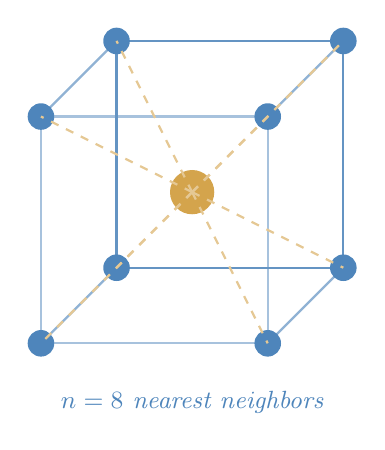
\begin{tikzpicture}[scale=1.6]
  % Draw a stylized BCC unit cell
  \def\a{1.8}
  % Back face
  \draw[bccblue!40, thick] (0,0) -- (\a,0) -- (\a,\a) -- (0,\a) -- cycle;
  % Front face
  \draw[bccblue!70, thick] (0.6,0.6) -- (\a+0.6,0.6) -- (\a+0.6,\a+0.6) -- (0.6,\a+0.6) -- cycle;
  % Connecting edges
  \draw[bccblue!50, thick] (0,0) -- (0.6,0.6);
  \draw[bccblue!50, thick] (\a,0) -- (\a+0.6,0.6);
  \draw[bccblue!50, thick] (\a,\a) -- (\a+0.6,\a+0.6);
  \draw[bccblue!50, thick] (0,\a) -- (0.6,\a+0.6);
  % Corner nodes
  \foreach \x/\y in {0/0, \a/0, \a/\a, 0/\a} {
    \fill[bccblue!80] (\x,\y) circle (3pt);
    \fill[bccblue!80] (\x+0.6,\y+0.6) circle (3pt);
  }
  % Center node (the body-centered atom)
  \fill[bccgold] (\a/2+0.3, \a/2+0.3) circle (5pt);
  % Bonds to center
  \foreach \x/\y in {0/0, \a/0, \a/\a, 0/\a,
                      0.6/0.6, \a+0.6/0.6, \a+0.6/\a+0.6, 0.6/\a+0.6} {
    \draw[bccgold!60, thick, dashed] (\a/2+0.3, \a/2+0.3) -- (\x,\y);
  }
  % Label
  \node[below, bccblue!80, font=\small\itshape] at (\a/2+0.3, -0.3) {$n = 8$ nearest neighbors};
\end{tikzpicture}

\vspace{1.5cm}

{\large Alan Garcia}\\[4pt]
{\normalsize Independent Researcher}\\[2pt]
{\small\texttt{alan.javier.garcia@gmail.com}}

\vspace{1cm}

{\normalsize February 2026}

\vspace{1.5cm}

\begin{minipage}{0.8\textwidth}\small\itshape
\centering
``What would have to be true for a photon to behave as both a wave and a particle?''\\[6pt]
This document summarizes the physical hypothesis underlying the Binary Singularity
Model (BSM): a framework in which fundamental constants emerge from the spectral
geometry of a body-centered cubic lattice. Two inputs---the BCC coordination number
$n = 8$ and the transcendental $\pi$---with spatial dimension $d = 3$ entering
higher-order formulas, produce six fundamental constants with zero free parameters.
\end{minipage}

\end{titlepage}

\tableofcontents
\newpage

% ══════════════════════════════════════════════════════════════
\section{Origin: The Photon as a Composite Object}
\label{sec:origin}

\begin{hypothesisbox}[Core Hypothesis]
The photon is a composite of two sub-Planck-scale singularities in helical orbit.
Viewed from the side, the orbit traces a wave; viewed head-on, it appears as a point.
Wave--particle duality emerges from the geometry of the binary orbit.
\end{hypothesisbox}

\noindent
The Binary Singularity Model began with a question about wave--particle duality:
what physical structure could produce both wave-like and particle-like behavior from
the same object? The proposed answer is a binary system of two gravitational
singularities orbiting each other at a scale far below the Planck length
($\ell_P \approx 1.6 \times 10^{-35}$~m). At such scales, the concept of
``probing with light'' breaks down---wavelengths short enough to resolve the
structure would carry enough energy to collapse into black holes---making the
sub-Planckian regime causally inaccessible to direct measurement.

\begin{figure}[H]
\centering
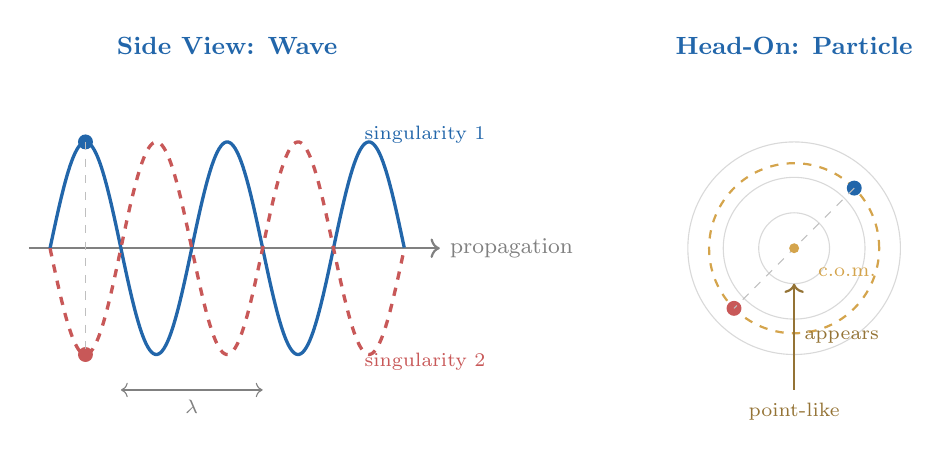
\begin{tikzpicture}[scale=0.9]
  % Helical orbit - side view
  \begin{scope}[xshift=-5cm]
    \node[above, font=\bfseries\small, bccblue] at (2.5,2.6) {Side View: Wave};
    \draw[->, gray, thick] (-0.3,0) -- (5.5,0) node[right, font=\footnotesize] {propagation};
    \draw[bccblue, very thick, smooth, samples=200, domain=0:5]
      plot (\x, {1.5*sin(360*\x/2.0)});
    \draw[bccred, very thick, smooth, samples=200, domain=0:5, dashed]
      plot (\x, {-1.5*sin(360*\x/2.0)});
    \fill[bccblue] (0.5, {1.5*sin(360*0.5/2.0)}) circle (3pt);
    \fill[bccred] (0.5, {-1.5*sin(360*0.5/2.0)}) circle (3pt);
    \draw[gray!50, thin, dashed] (0.5, {1.5*sin(360*0.5/2.0)})
      -- (0.5, {-1.5*sin(360*0.5/2.0)});
    \node[bccblue, font=\scriptsize, right] at (4.3, 1.6) {singularity 1};
    \node[bccred, font=\scriptsize, right] at (4.3, -1.6) {singularity 2};
    \draw[<->, gray, thin] (1.0, -2.0) -- (3.0, -2.0)
      node[midway, below, font=\scriptsize] {$\lambda$};
  \end{scope}
  % Head-on view
  \begin{scope}[xshift=4cm]
    \node[above, font=\bfseries\small, bccblue] at (1.5,2.6) {Head-On: Particle};
    \draw[gray!30, thin] (1.5,0) circle (1.5);
    \draw[gray!30, thin] (1.5,0) circle (1.0);
    \draw[gray!30, thin] (1.5,0) circle (0.5);
    \draw[bccgold, thick, dashed] (1.5,0) circle (1.2);
    \fill[bccblue] (1.5+1.2*0.707, 1.2*0.707) circle (3pt);
    \fill[bccred] (1.5-1.2*0.707, -1.2*0.707) circle (3pt);
    \draw[gray!50, thin, dashed] (1.5+1.2*0.707, 1.2*0.707)
      -- (1.5-1.2*0.707, -1.2*0.707);
    \fill[bccgold] (1.5,0) circle (2pt);
    \node[bccgold, font=\scriptsize, below right] at (1.7,-0.15) {c.o.m.};
    \draw[->, thick, bccgold!70!black] (1.5, -2.0) -- (1.5, -0.5)
      node[midway, right, font=\scriptsize] {appears};
    \node[font=\scriptsize, bccgold!70!black] at (1.5, -2.3) {point-like};
  \end{scope}
\end{tikzpicture}
\caption{The binary singularity hypothesis. Two sub-Planckian singularities in
helical orbit appear as a wave (side view) or a particle (head-on). The wavelength
$\lambda$ and energy $E = hc/\lambda$ are determined by the orbital parameters.}
\label{fig:photon-composite}
\end{figure}

The self-consistency requirement---that such a binary system respect both quantum
mechanics and general relativity at its own scale---forces structural constraints.
Over iterative computation, these constraints converged on a body-centered cubic
(BCC) lattice as the underlying spatial geometry. The BSM framework then identifies
all particles as topological defects on this lattice, and the photon as the
longitudinal propagation mode of the binary defect.

% ══════════════════════════════════════════════════════════════
\section{The BCC Lattice}
\label{sec:bcc}

The body-centered cubic lattice is defined by corner sites plus a central site
in each cubic unit cell. Each site has $n = 8$ nearest neighbors (coordination
number). This is the fundamental input of the BSM framework.

\begin{figure}[H]
\centering
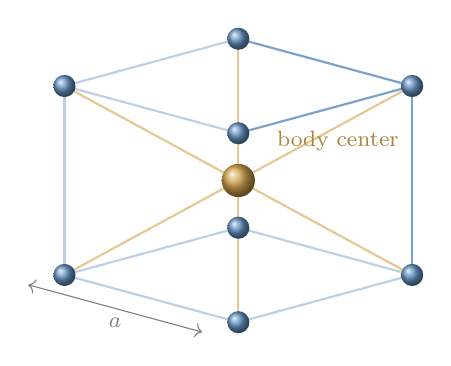
\begin{tikzpicture}[scale=1.0,
  x={(0.92cm,-0.25cm)}, y={(0.92cm,0.25cm)}, z={(0cm,1.0cm)}]
  \def\L{2.4}
  % Back edges
  \draw[bccblue!30, thick] (0,0,0) -- (\L,0,0);
  \draw[bccblue!30, thick] (0,0,0) -- (0,\L,0);
  \draw[bccblue!30, thick] (0,0,0) -- (0,0,\L);
  \draw[bccblue!30, thick] (\L,0,0) -- (\L,\L,0);
  \draw[bccblue!30, thick] (0,\L,0) -- (\L,\L,0);
  \draw[bccblue!30, thick] (\L,0,0) -- (\L,0,\L);
  \draw[bccblue!30, thick] (0,\L,0) -- (0,\L,\L);
  \draw[bccblue!30, thick] (0,0,\L) -- (\L,0,\L);
  \draw[bccblue!30, thick] (0,0,\L) -- (0,\L,\L);
  \draw[bccblue!60, thick] (\L,\L,0) -- (\L,\L,\L);
  \draw[bccblue!60, thick] (\L,0,\L) -- (\L,\L,\L);
  \draw[bccblue!60, thick] (0,\L,\L) -- (\L,\L,\L);
  % Center-to-corner bonds
  \foreach \x in {0,\L} \foreach \y in {0,\L} \foreach \z in {0,\L} {
    \draw[bccgold!60, thick] (\L/2,\L/2,\L/2) -- (\x,\y,\z);
  }
  % Corner atoms
  \foreach \x in {0,\L} \foreach \y in {0,\L} \foreach \z in {0,\L} {
    \shade[ball color=bccblue!70] (\x,\y,\z) circle (4pt);
  }
  % Center atom
  \shade[ball color=bccgold] (\L/2,\L/2,\L/2) circle (6pt);
  \node[font=\footnotesize, bccgold!80!black, right] at (\L/2+0.2,\L/2+0.2,\L/2+0.5)
    {body center};
  \draw[<->, gray, thin] (0,-0.5,0) -- (\L,-0.5,0)
    node[midway, below, font=\footnotesize] {$a$};
\end{tikzpicture}
\hspace{1.5cm}
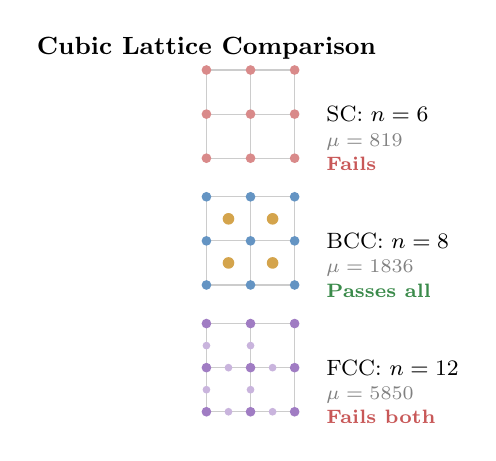
\begin{tikzpicture}[scale=0.7]
  \node[font=\bfseries\small] at (0,5.5) {Cubic Lattice Comparison};
  \begin{scope}[yshift=3.5cm]
    \draw[gray!40] (0,0) grid[step=0.8] (1.6,1.6);
    \foreach \x in {0,0.8,1.6} \foreach \y in {0,0.8,1.6}
      \fill[bccred!70] (\x,\y) circle (2.5pt);
    \node[font=\footnotesize, right] at (2.0, 0.8) {SC: $n=6$};
    \node[font=\scriptsize, right, gray] at (2.0, 0.3) {$\mu = 819$};
    \node[font=\scriptsize, right, bccred] at (2.0, -0.1) {\textbf{Fails}};
  \end{scope}
  \begin{scope}[yshift=1.2cm]
    \draw[gray!40] (0,0) grid[step=0.8] (1.6,1.6);
    \foreach \x in {0,0.8,1.6} \foreach \y in {0,0.8,1.6}
      \fill[bccblue!70] (\x,\y) circle (2.5pt);
    \foreach \x in {0.4,1.2} \foreach \y in {0.4,1.2}
      \fill[bccgold] (\x,\y) circle (3pt);
    \node[font=\footnotesize, right] at (2.0, 0.8) {BCC: $n=8$};
    \node[font=\scriptsize, right, gray] at (2.0, 0.3) {$\mu = 1836$};
    \node[font=\scriptsize, right, bccgreen] at (2.0, -0.1) {\textbf{Passes all}};
  \end{scope}
  \begin{scope}[yshift=-1.1cm]
    \draw[gray!40] (0,0) grid[step=0.8] (1.6,1.6);
    \foreach \x in {0,0.8,1.6} \foreach \y in {0,0.8,1.6}
      \fill[bccpurple!70] (\x,\y) circle (2.5pt);
    \foreach \x in {0,0.8} \foreach \y in {0,0.8} {
      \fill[bccpurple!40] (\x+0.4,\y) circle (2pt);
      \fill[bccpurple!40] (\x,\y+0.4) circle (2pt);
    }
    \node[font=\footnotesize, right] at (2.0, 0.8) {FCC: $n=12$};
    \node[font=\scriptsize, right, gray] at (2.0, 0.3) {$\mu = 5850$};
    \node[font=\scriptsize, right, bccred] at (2.0, -0.1) {\textbf{Fails both}};
  \end{scope}
\end{tikzpicture}
\caption{\textbf{Left:} The BCC unit cell. Eight corner sites (blue) each share
$1/8$ with adjacent cells; the body-center site (gold) belongs entirely to this cell.
Each site has $n = 8$ nearest neighbors. \textbf{Right:} Only BCC ($n = 8$) yields
the correct mass generator $\mu = 1836 \approx m_p/m_e$.}
\label{fig:bcc-lattice}
\end{figure}

\subsection{Why BCC?}

The tree-level proton--electron mass generator $\mu(n) = \frac{3}{2}\sigma(n)\cdot\rho(n)$
uniquely selects BCC. Simple cubic ($n = 6$) gives $\mu = 819$, which is 55\% below
the experimental proton mass ratio. FCC ($n = 12$) gives $\mu = 5850$, which is 219\%
too high. No perturbative correction can bridge these gaps. The BCC lattice is the
\emph{only} cubic lattice whose coordination number yields both $\tau(8) = 137$ and
$\mu(8) = 1836$.

% ══════════════════════════════════════════════════════════════
\section{Generator Functions from SO(3) Representation Theory}
\label{sec:generators}

Four generator functions of the coordination number $n$, arising from the
representation theory of $\mathrm{SO}(3)$, build all observable quantities:

\begin{insightbox}[The Four Generators]
\begin{align}
  \tau(n) &= n(2n+1) + 1 \quad &&\text{(topological: } \dim \Lambda^2 D(n) \oplus D(0)\text{)} \label{eq:tau}\\
  \sigma(n) &= n(2n+1) \quad &&\text{(pairwise: } \tbinom{2n+1}{2}\text{ substate couplings)} \label{eq:sigma}\\
  \rho(n) &= n+1 \quad &&\text{(radial: shells in spin-}n\text{ representation)} \label{eq:rho}\\
  \mu(n) &= \tfrac{3}{2}\,\sigma(n)\,\rho(n) \quad &&\text{(mass: composite generator)} \label{eq:mu}
\end{align}
\end{insightbox}

\noindent
At $n = 8$: $\tau = 137$, $\sigma = 136$, $\rho = 9$, $\mu = 1836$.

\begin{figure}[H]
\centering
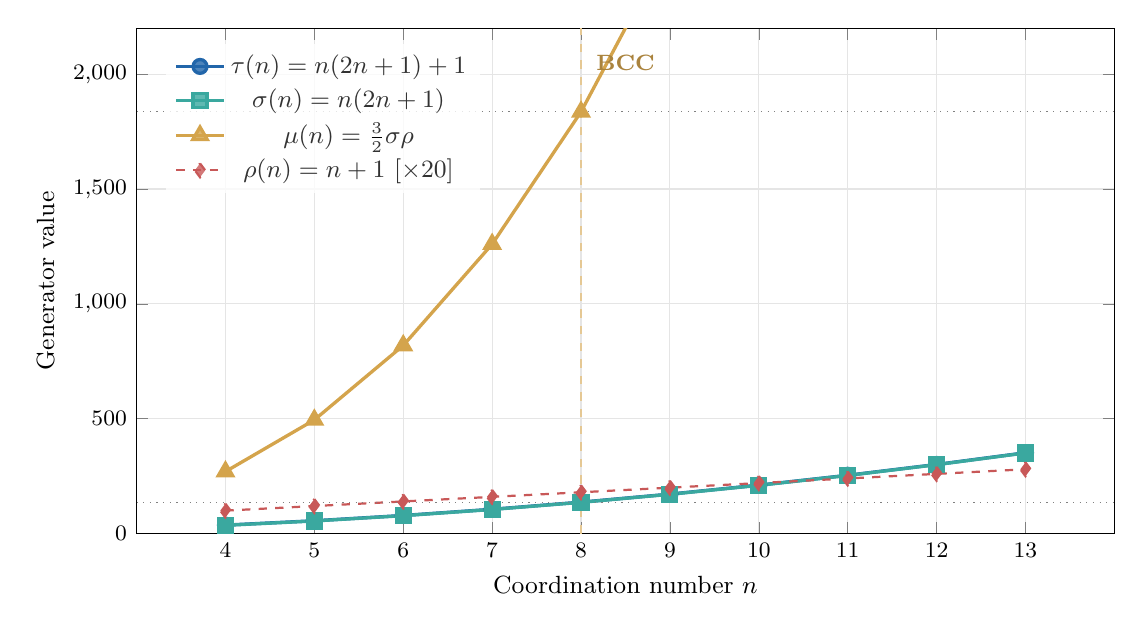
\begin{tikzpicture}
\begin{axis}[
  width=14cm, height=8cm,
  xlabel={Coordination number $n$},
  ylabel={Generator value},
  xmin=3, xmax=14, ymin=0, ymax=2200,
  xtick={4,5,6,7,8,9,10,11,12,13},
  legend pos=north west,
  legend style={font=\small, draw=none, fill=white, fill opacity=0.8},
  grid=major, grid style={gray!20},
  every axis label/.style={font=\small},
  tick label style={font=\footnotesize}
]
  \addplot[bccblue, very thick, mark=*, mark size=2.5, samples at={4,5,...,13}]
    {x*(2*x+1)+1};
  \addlegendentry{$\tau(n) = n(2n+1)+1$}
  \addplot[bccteal, very thick, mark=square*, mark size=2.5, samples at={4,5,...,13}]
    {x*(2*x+1)};
  \addlegendentry{$\sigma(n) = n(2n+1)$}
  \addplot[bccgold, very thick, mark=triangle*, mark size=3, samples at={4,5,...,13}]
    {1.5*x*(2*x+1)*(x+1)};
  \addlegendentry{$\mu(n) = \tfrac{3}{2}\sigma\rho$}
  \addplot[bccred, thick, mark=diamond*, mark size=2.5, dashed, samples at={4,5,...,13}]
    {(x+1)*20};
  \addlegendentry{$\rho(n) = n+1$ [$\times 20$]}
  \draw[bccgold!60, thick, dashed] (axis cs:8,0) -- (axis cs:8,2200);
  \node[font=\footnotesize\bfseries, bccgold!80!black] at (axis cs:8.5,2050) {BCC};
  \draw[gray, thin, dotted] (axis cs:3,137) -- (axis cs:14,137)
    node[right, font=\scriptsize] {$137$};
  \draw[gray, thin, dotted] (axis cs:3,1836) -- (axis cs:14,1836)
    node[right, font=\scriptsize] {$1836$};
\end{axis}
\end{tikzpicture}
\caption{The four BSM generator functions versus coordination number $n$. At $n = 8$
(BCC, dashed gold line), $\tau = 137 \approx \ainv$ and $\mu = 1836 \approx m_p/m_e$.
The horizontal dotted lines mark the experimental values.}
\label{fig:generators}
\end{figure}

% ══════════════════════════════════════════════════════════════
\section{Particles as Lattice Defects}
\label{sec:defects}

In the BSM framework, every particle is a topological defect---a localized
disturbance in the BCC lattice. The defect classification determines the particle
spectrum.

\begin{figure}[H]
\centering
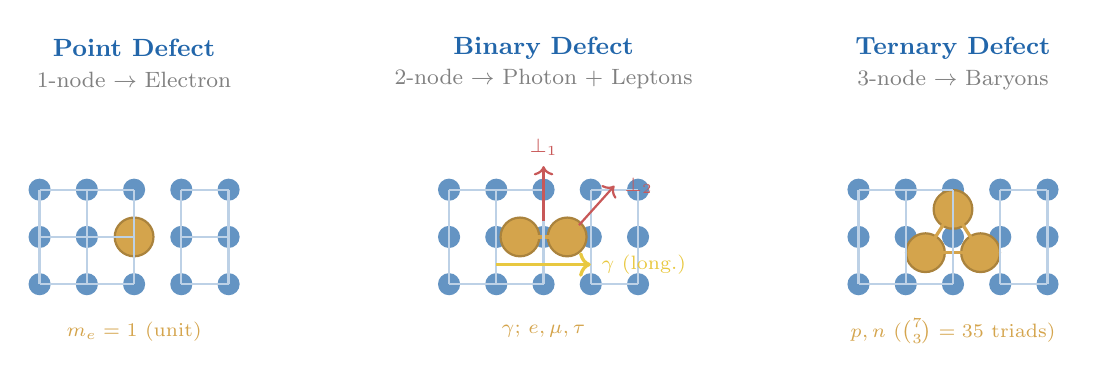
\begin{tikzpicture}[
  node/.style={circle, fill=bccblue!70, inner sep=0pt, minimum size=8pt},
  defect/.style={circle, fill=bccgold, inner sep=0pt, minimum size=10pt,
    draw=bccgold!80!black, thick},
  bond/.style={bccblue!30, thick},
  dbond/.style={bccgold, very thick}
]
% ── Point defect (electron) ──────────────────────
\begin{scope}[xshift=-5.2cm]
  \node[font=\bfseries\small, bccblue] at (0, 2.4) {Point Defect};
  \node[font=\footnotesize, gray] at (0, 2.0) {1-node $\to$ Electron};
  \foreach \x in {-1.2,-0.6,0,0.6,1.2} \foreach \y in {-0.6,0,0.6} {
    \node[node] at (\x,\y) {};
  }
  \node[defect, minimum size=14pt] at (0,0) {};
  \foreach \x in {-1.2,-0.6,0.6} {
    \draw[bond] (\x,-0.6) -- (\x+0.6,-0.6);
    \draw[bond] (\x,0) -- (\x+0.6,0);
    \draw[bond] (\x,0.6) -- (\x+0.6,0.6);
  }
  \foreach \x in {-1.2,-0.6,0,0.6,1.2} {
    \draw[bond] (\x,-0.6) -- (\x,0);
    \draw[bond] (\x,0) -- (\x,0.6);
  }
  \node[font=\scriptsize, bccgold] at (0, -1.2) {$m_e = 1$ (unit)};
\end{scope}
% ── Binary defect (leptons + photon) ─────────────
\begin{scope}[xshift=0cm]
  \node[font=\bfseries\small, bccblue] at (0, 2.4) {Binary Defect};
  \node[font=\footnotesize, gray] at (0, 2.0) {2-node $\to$ Photon + Leptons};
  \foreach \x in {-1.2,-0.6,0,0.6,1.2} \foreach \y in {-0.6,0,0.6} {
    \node[node] at (\x,\y) {};
  }
  \node[defect, minimum size=14pt] at (-0.3,0) {};
  \node[defect, minimum size=14pt] at (0.3,0) {};
  \draw[dbond] (-0.3,0) -- (0.3,0);
  \foreach \x in {-1.2,-0.6,0.6} {
    \draw[bond] (\x,-0.6) -- (\x+0.6,-0.6);
    \draw[bond] (\x,0.6) -- (\x+0.6,0.6);
  }
  \foreach \x in {-1.2,-0.6,0,0.6,1.2} {
    \draw[bond] (\x,-0.6) -- (\x,0);
    \draw[bond] (\x,0) -- (\x,0.6);
  }
  % Longitudinal arrow (photon)
  \draw[->, photonyellow, very thick] (-0.6, -0.35) -- (0.6, -0.35)
    node[right, font=\scriptsize] {$\gamma$ (long.)};
  % Transverse arrows (leptons)
  \draw[->, bccred, thick] (0, 0.2) -- (0, 0.9)
    node[above, font=\scriptsize] {$\perp_1$};
  \draw[->, bccred, thick] (0.45, 0.15) -- (0.9, 0.65)
    node[right, font=\scriptsize] {$\perp_2$};
  \node[font=\scriptsize, bccgold] at (0, -1.2) {$\gamma$; $e, \mu, \tau$};
\end{scope}
% ── Ternary defect (proton/neutron) ──────────────
\begin{scope}[xshift=5.2cm]
  \node[font=\bfseries\small, bccblue] at (0, 2.4) {Ternary Defect};
  \node[font=\footnotesize, gray] at (0, 2.0) {3-node $\to$ Baryons};
  \foreach \x in {-1.2,-0.6,0,0.6,1.2} \foreach \y in {-0.6,0,0.6} {
    \node[node] at (\x,\y) {};
  }
  \node[defect, minimum size=14pt] at (-0.35,-0.2) {};
  \node[defect, minimum size=14pt] at (0.35,-0.2) {};
  \node[defect, minimum size=14pt] at (0,0.35) {};
  \draw[dbond] (-0.35,-0.2) -- (0.35,-0.2);
  \draw[dbond] (0.35,-0.2) -- (0,0.35);
  \draw[dbond] (0,0.35) -- (-0.35,-0.2);
  \foreach \x in {-1.2,-0.6,0.6} {
    \draw[bond] (\x,-0.6) -- (\x+0.6,-0.6);
    \draw[bond] (\x,0.6) -- (\x+0.6,0.6);
  }
  \foreach \x in {-1.2,-0.6,0,0.6,1.2} {
    \draw[bond] (\x,-0.6) -- (\x,0);
    \draw[bond] (\x,0) -- (\x,0.6);
  }
  \node[font=\scriptsize, bccgold] at (0, -1.2) {$p, n$ ($\binom{7}{3}=35$ triads)};
\end{scope}
\end{tikzpicture}
\caption{The BSM defect classification. The \textbf{binary defect} (2-node line)
hosts the photon as its longitudinal mode (yellow arrow) and the three lepton
generations as transverse excitations (red arrows). The \textbf{ternary defect}
(3-node triangle) embeds in $\binom{n-1}{d} = 35$ orientational triads.}
\label{fig:defects}
\end{figure}


% ══════════════════════════════════════════════════════════════
\section{The Photon on the BCC Lattice}
\label{sec:photon}

The photon is the best-characterized object in the BSM framework: its dressed
propagator yields $\ainv = 137.035\,999\,177$, matching CODATA to $< 0.001\ppb$.
This section consolidates the photon's geometric identity, field-theoretic
interpretation, dispersion relation, and observational constraints.

\subsection{Geometric Identity: Longitudinal Mode of the Binary Defect}

A bond in $d$ dimensions decomposes into:
\begin{itemize}[nosep,leftmargin=1.5em]
  \item 1 longitudinal direction (along the bond) $\longrightarrow$ \textbf{photon}
  \item $d-1 = 2$ transverse directions (normal to the bond) $\longrightarrow$
    \textbf{charged leptons} ($e, \mu, \tau$)
\end{itemize}

\noindent
The Koide parameter $Q = (d-1)/d = 2/3$ counts the transverse fraction. The photon
occupies the remaining $1/d$ fraction.

\begin{figure}[H]
\centering
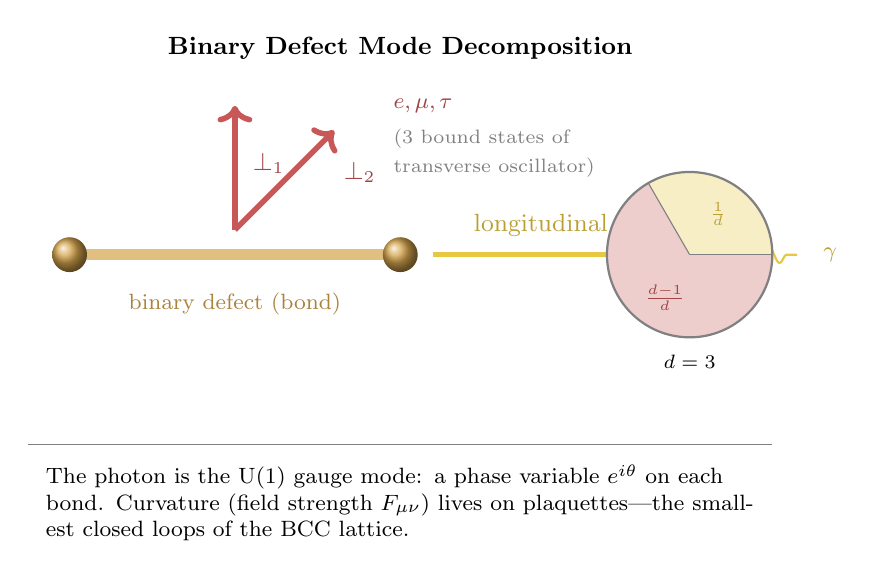
\begin{tikzpicture}[scale=1.05]
  % ── The binary defect decomposition ──
  \node[font=\bfseries\small] at (5, 4.5) {Binary Defect Mode Decomposition};

  % The bond
  \draw[bccgold, line width=4pt, opacity=0.7] (1,2) -- (5,2);
  \shade[ball color=bccgold] (1,2) circle (6pt);
  \shade[ball color=bccgold] (5,2) circle (6pt);
  \node[font=\footnotesize, bccgold!80!black] at (3, 1.4) {binary defect (bond)};

  % Longitudinal: photon
  \draw[->, photonyellow, line width=2pt] (5.4, 2) -- (8, 2);
  \node[font=\small, photonyellow!80!black, above] at (6.7, 2.1) {longitudinal};
  % Wavy photon symbol
  \draw[photonyellow, thick, decorate, decoration={snake, amplitude=3pt, segment length=8pt}]
    (8.3, 2) -- (9.8, 2);
  \node[font=\footnotesize, photonyellow!80!black, right] at (10, 2) {$\gamma$};

  % Transverse 1: leptons
  \draw[->, bccred, line width=2pt] (3, 2.3) -- (3, 3.8);
  \node[font=\small, bccred!80!black, right] at (3.1, 3.1) {$\perp_1$};
  % Transverse 2
  \draw[->, bccred, line width=2pt] (3, 2.3) -- (4.2, 3.5);
  \node[font=\small, bccred!80!black, right] at (4.2, 3.0) {$\perp_2$};

  % Lepton labels
  \node[font=\footnotesize, bccred!80!black, right] at (4.8, 3.8) {$e, \mu, \tau$};
  \node[font=\scriptsize, gray, right] at (4.8, 3.4)
    {(3 bound states of};
  \node[font=\scriptsize, gray, right] at (4.8, 3.05)
    {transverse oscillator)};

  % Fraction diagram
  \begin{scope}[xshift=8.5cm, yshift=2cm]
    \fill[photonyellow!30] (0,0) -- (0:1.0) arc (0:120:1.0) -- cycle;
    \fill[bccred!30] (0,0) -- (120:1.0) arc (120:360:1.0) -- cycle;
    \draw[thick, gray] (0,0) circle (1.0);
    \draw[gray] (0,0) -- (0:1.0);
    \draw[gray] (0,0) -- (120:1.0);
    \node[font=\scriptsize, photonyellow!80!black] at (55:0.6) {$\frac{1}{d}$};
    \node[font=\scriptsize, bccred!80!black] at (240:0.6) {$\frac{d{-}1}{d}$};
    \node[font=\scriptsize] at (0, -1.3) {$d = 3$};
  \end{scope}

  % U(1) gauge interpretation
  \begin{scope}[yshift=-0.3cm]
    \draw[gray, thin] (0.5, 0) -- (9.5, 0);
    \node[font=\footnotesize, align=left, text width=9cm] at (5, -0.7)
      {The photon is the $\mathrm{U}(1)$ gauge mode: a phase variable $e^{i\theta}$
       on each bond. Curvature (field strength $F_{\mu\nu}$) lives on plaquettes---the
       smallest closed loops of the BCC lattice.};
  \end{scope}
\end{tikzpicture}
\caption{The binary defect decomposes into a longitudinal mode (the photon, $1/d$
of degrees of freedom) and transverse modes (the leptons, $(d-1)/d$ of degrees of
freedom). In $d=3$: 1 photon direction, 2 transverse directions hosting 3 lepton
generations.}
\label{fig:photon-decomposition}
\end{figure}

\subsection{The Dyson Equation as the Photon's Self-Energy}

The BSM formula for $\ainv$ is interpreted as a dressed photon propagator:
\begin{equation}
\boxed{
  \ainv = B + \frac{1}{(n{+}2)\,B^2}
}, \qquad
B = \tau + \frac{c_1}{\tau} - \frac{1}{2\tau^2}
  - \frac{1}{(n{-}1)\tau^3} + \frac{c_4}{\tau^4}
\label{eq:alpha}
\end{equation}

\noindent
with $c_1 = \pi^2/2$ (Brillouin zone integral), $c_4 = \frac{18}{17}\pi^3$
(spectral skewness). The lattice parameters are coupling $g^2 = 1/2$ and Dirac
multiplicity $N_D = 4$. This has the structure of a Dyson equation
$G^{-1} = G_0^{-1} - \Sigma(G)$, where the loop coefficients encode the
BCC geometry as seen by the photon.

\begin{figure}[H]
\centering
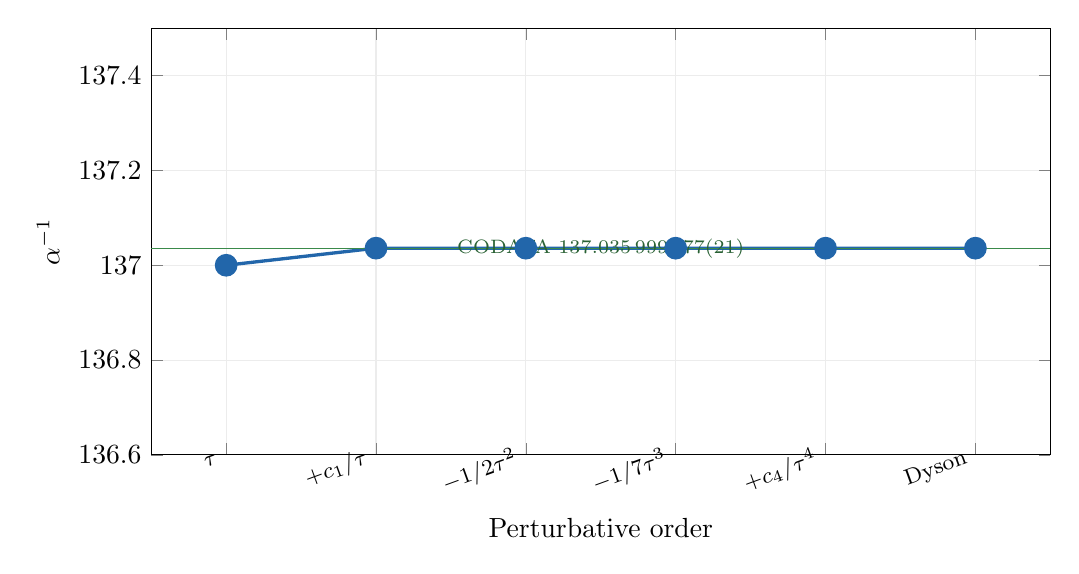
\begin{tikzpicture}
\begin{axis}[
  width=13cm, height=7cm,
  xlabel={Perturbative order},
  ylabel={$\ainv$},
  ymin=136.6, ymax=137.5,
  xmin=0.5, xmax=6.5,
  xtick={1,2,3,4,5,6},
  xticklabels={$\tau$, $+c_1/\tau$, $-1/2\tau^2$, $-1/7\tau^3$, $+c_4/\tau^4$, Dyson},
  x tick label style={font=\footnotesize, rotate=20, anchor=east},
  legend pos=north east,
  legend style={font=\small, draw=none},
  grid=major, grid style={gray!15}
]
  \addplot[bccblue, very thick, mark=*, mark size=3.5] coordinates {
    (1, 137)
    (2, 137.036044944)
    (3, 137.036018311)
    (4, 137.036017570)
    (5, 137.035999078)
    (6, 137.035999177)
  };
  \addplot[name path=upper, draw=none] coordinates {(0.5,137.036000) (6.5,137.036000)};
  \addplot[name path=lower, draw=none] coordinates {(0.5,137.035998) (6.5,137.035998)};
  \addplot[bccgreen!20] fill between[of=upper and lower];
  \draw[bccgreen, thin] (axis cs:0.5,137.035999177) -- (axis cs:6.5,137.035999177);
  \node[font=\scriptsize, bccgreen!70!black] at (axis cs:3.5, 137.036005)
    {CODATA $137.035\,999\,177(21)$};
\end{axis}
\end{tikzpicture}
\caption{Convergence of $\ainv$ as successive perturbative corrections are added.
The tree level $\tau = 137$ is corrected order-by-order; the final Dyson resummation
yields agreement with CODATA to $< 0.001\ppb$.}
\label{fig:alpha-convergence}
\end{figure}

\subsection{Complex Structure of the Dyson Cubic}

The Dyson equation is a cubic $z^3 - Bz^2 - 1/(n{+}2) = 0$ with discriminant
$\Delta < 0$: one real root $z_1 = \ainv$ and a complex conjugate pair
$z_{2,3} \approx \pm 0.027\,i$. By Vieta's formulas, $|z_{2,3}|^2 = \alpha/(n+2)$,
so the complex roots have modulus $\sim\sqrt{\alpha}$. The physical coupling is
separated from the complex pair by $\ainv/|z_2| \approx 5000$.

\begin{figure}[H]
\centering
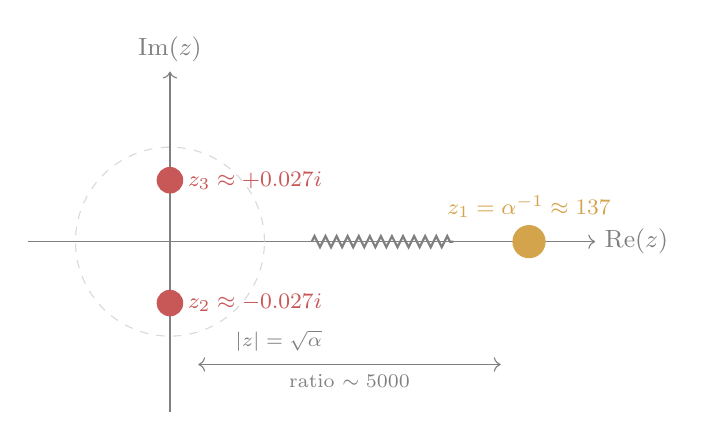
\begin{tikzpicture}[scale=1.2]
  \draw[->, gray] (-1.5,0) -- (4.5,0) node[right, font=\small] {Re$(z)$};
  \draw[->, gray] (0,-1.8) -- (0,1.8) node[above, font=\small] {Im$(z)$};
  \fill[bccred] (0, 0.65) circle (4pt)
    node[right, font=\footnotesize, xshift=3pt] {$z_3 \approx +0.027i$};
  \fill[bccred] (0, -0.65) circle (4pt)
    node[right, font=\footnotesize, xshift=3pt] {$z_2 \approx -0.027i$};
  \fill[bccgold] (3.8, 0) circle (5pt);
  \node[bccgold, font=\footnotesize, above] at (3.8, 0.15) {$z_1 = \ainv \approx 137$};
  \draw[<->, gray, thin] (0.3, -1.3) -- (3.5, -1.3)
    node[midway, below, font=\scriptsize] {ratio $\sim 5000$};
  \draw[gray!30, dashed] (0,0) circle (1.0);
  \node[font=\scriptsize, gray] at (1.15, -1.05) {$|z|=\sqrt{\alpha}$};
  \draw[gray, thick, decorate, decoration={zigzag, segment length=4pt, amplitude=2pt}]
    (1.5, 0) -- (3.0, 0);
\end{tikzpicture}
\caption{Complex roots of the BSM Dyson cubic. The physical root $\ainv \approx 137$
lies far from the complex pair $|z_{2,3}| \sim \sqrt{\alpha}$, confirming deep
perturbative stability.}
\label{fig:complex-alpha}
\end{figure}


\subsection{Lattice Dispersion Relation}
\label{sec:dispersion}

On any lattice with spacing $a$, the photon dispersion relation in the
tight-binding approximation is:
\begin{equation}
\boxed{
  \omega(k) = \frac{2c}{a}\left|\sin\!\left(\frac{ka}{2}\right)\right|
}
\label{eq:dispersion}
\end{equation}

\noindent
At long wavelengths ($ka \ll 1$), this recovers $\omega = ck$ with corrections of
order $(ka)^2$. The group velocity is
$v_g = c\cos(ka/2) = c[1 - (ka)^2/8 + \cdots]$.

\begin{figure}[H]
\centering
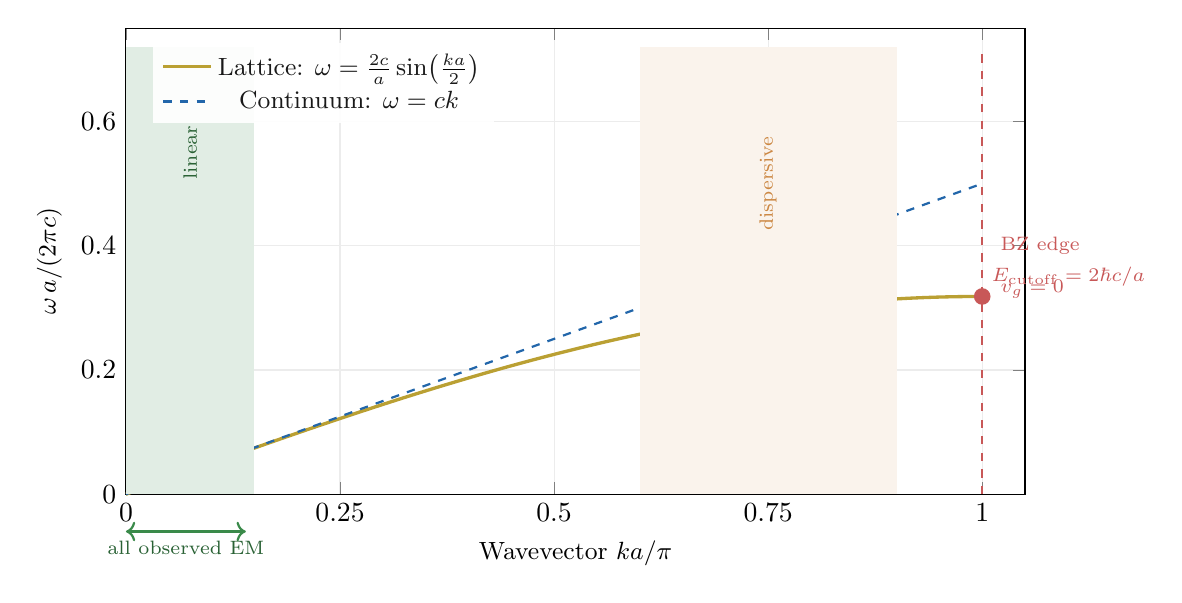
\begin{tikzpicture}
\begin{axis}[
  width=13cm, height=7.5cm,
  xlabel={Wavevector $ka/\pi$},
  ylabel={$\omega\,a/(2\pi c)$},
  xmin=0, xmax=1.05,
  ymin=0, ymax=0.75,
  xtick={0, 0.25, 0.5, 0.75, 1.0},
  legend pos=north west,
  legend style={font=\small, draw=none, fill=white, fill opacity=0.9},
  grid=major, grid style={gray!15},
  every axis label/.style={font=\small},
  clip=false
]
  % Lattice dispersion: omega = (2c/a)|sin(ka/2)|
  % With x = ka/pi, we have ka/2 = pi*x/2, so sin(ka/2) = sin(pi*x/2)
  % omega*a/(2*pi*c) = (1/pi)*sin(pi*x/2)
  \addplot[photonyellow!80!black, very thick, smooth, domain=0:1, samples=100]
    {(1/pi)*sin(deg(pi*x/2))};
  \addlegendentry{Lattice: $\omega = \frac{2c}{a}\sin\!\left(\frac{ka}{2}\right)$}

  % Continuum (linear)
  \addplot[bccblue, thick, dashed, domain=0:1, samples=50]
    {x/2};
  \addlegendentry{Continuum: $\omega = ck$}

  % Three regimes
  % Linear regime
  \fill[bccgreen!15] (axis cs:0,0) rectangle (axis cs:0.15,0.72);
  \node[font=\scriptsize, bccgreen!70!black, rotate=90] at (axis cs:0.075,0.55) {linear};

  % Dispersive regime
  \fill[vpcol!10] (axis cs:0.6,0) rectangle (axis cs:0.9,0.72);
  \node[font=\scriptsize, vpcol, rotate=90] at (axis cs:0.75,0.5) {dispersive};

  % BZ edge
  \draw[bccred, thick, dashed] (axis cs:1.0,0) -- (axis cs:1.0,0.72);
  \node[font=\scriptsize, bccred, right] at (axis cs:1.01, 0.4) {BZ edge};
  \node[font=\scriptsize, bccred, right] at (axis cs:1.01, 0.33) {$v_g = 0$};

  % Standing wave marker
  \fill[bccred] (axis cs:1.0, {(1/pi)*sin(deg(pi*1.0/2))}) circle (3pt);
  \node[font=\scriptsize, bccred, above right] at (axis cs:1.0, {(1/pi)})
    {$E_{\mathrm{cutoff}} = 2\hbar c/a$};

  % Annotation: all observed photons
  \draw[<->, bccgreen, thick] (axis cs:0, -0.06) -- (axis cs:0.14, -0.06);
  \node[font=\scriptsize, bccgreen!70!black, below] at (axis cs:0.07, -0.06)
    {all observed EM};

\end{axis}
\end{tikzpicture}
\caption{The lattice dispersion relation $\omega(k)$ (solid gold) versus the continuum
linear relation $\omega = ck$ (dashed blue). Three regimes emerge: a linear regime
($ka \ll 1$, indistinguishable from continuum), a dispersive regime ($ka \sim 1$,
$v_g < c$), and the Brillouin zone edge ($k = \pi/a$, standing wave, $v_g = 0$).
\emph{All observed electromagnetic radiation} occupies the green band at the far left.}
\label{fig:dispersion}
\end{figure}


\subsection{Group Velocity and Vacuum Dispersion}

The lattice predicts a phenomenon absent from continuum QED: \emph{vacuum dispersion}.
High-energy photons travel slightly slower than low-energy ones:
\begin{equation}
  \frac{\Delta v}{c} = 1 - \cos\!\left(\frac{ka}{2}\right)
  \approx \frac{1}{2}\left(\frac{Ea}{4\pi\hbar c}\right)^{\!2}
\label{eq:vacdisp}
\end{equation}

\begin{figure}[H]
\centering
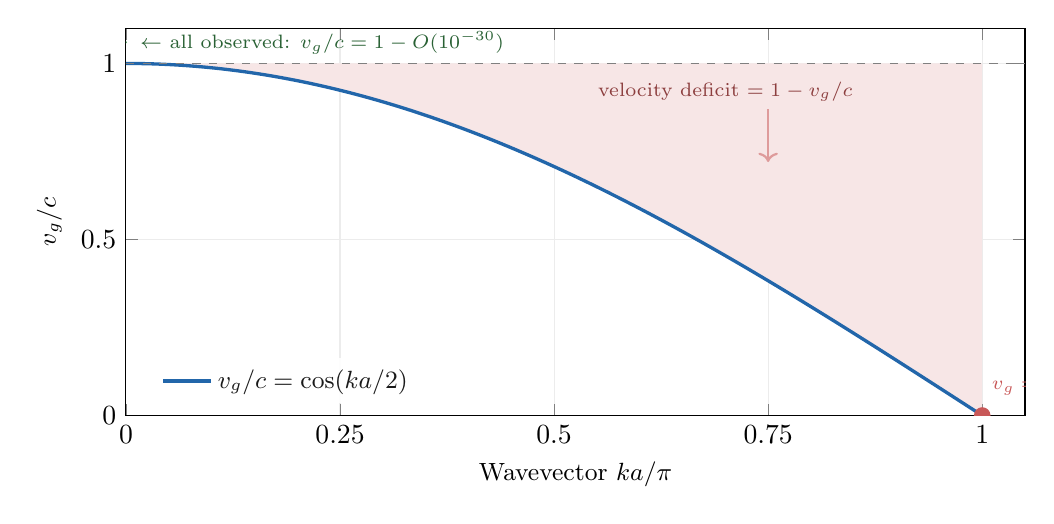
\begin{tikzpicture}
\begin{axis}[
  width=13cm, height=6.5cm,
  xlabel={Wavevector $ka/\pi$},
  ylabel={$v_g / c$},
  xmin=0, xmax=1.05,
  ymin=0, ymax=1.1,
  xtick={0, 0.25, 0.5, 0.75, 1.0},
  grid=major, grid style={gray!15},
  every axis label/.style={font=\small},
  legend pos=south west,
  legend style={font=\small, draw=none, fill=white, fill opacity=0.9},
]
  % v_g = cos(ka/2) = cos(pi*x/2)
  \addplot[bccblue, very thick, smooth, domain=0:1, samples=100]
    {cos(deg(pi*x/2))};
  \addlegendentry{$v_g/c = \cos(ka/2)$}

  % Reference line at c
  \addplot[gray, thin, dashed, domain=0:1.05] {1};

  % Shade the deficit area
  \addplot[name path=vg, draw=none, domain=0:1, samples=100]
    {cos(deg(pi*x/2))};
  \addplot[name path=one, draw=none, domain=0:1] {1};
  \addplot[bccred!15] fill between[of=one and vg];

  % Annotations
  \node[font=\scriptsize, bccred!70!black] at (axis cs:0.7, 0.92)
    {velocity deficit $= 1 - v_g/c$};
  \draw[->, bccred!60, thick] (axis cs:0.75, 0.87) -- (axis cs:0.75, 0.72);

  % Zero point
  \fill[bccred] (axis cs:1.0, 0) circle (3pt);
  \node[font=\scriptsize, bccred, above right] at (axis cs:1.0, 0.03)
    {$v_g = 0$};

  % Observed regime
  \draw[<->, bccgreen, thick] (axis cs:0.0, 1.06) -- (axis cs:0.001, 1.06);
  \node[font=\scriptsize, bccgreen!70!black, right] at (axis cs:0.005, 1.06)
    {$\leftarrow$ all observed: $v_g/c = 1 - O(10^{-30})$};
\end{axis}
\end{tikzpicture}
\caption{Group velocity $v_g/c = \cos(ka/2)$ on the lattice. The shaded area shows the
velocity deficit. At the Brillouin zone edge, $v_g \to 0$ and the photon becomes a
standing wave. For all observed electromagnetic radiation, the deviation from $c$ is
below $10^{-30}$---far beyond any conceivable measurement.}
\label{fig:group-velocity}
\end{figure}


\subsection{The Electromagnetic Spectrum on the Lattice}

The lattice becomes visible only at trans-Planckian energies. Assuming the
natural sub-Planckian spacing $a = \ell_P / \tau \approx 1.18 \times 10^{-37}$~m:

\begin{table}[H]
\centering\small
\begin{tabular}{lcccc}
\toprule
\textbf{Radiation} & \textbf{Energy} & $ka/2$ & \textbf{Dispersion} & $1 - v_g/c$ \\
\midrule
Radio (FM)        & $\sim\!10^{-7}$ eV  & $\sim\!10^{-37}$ & none & $< 10^{-73}$ \\
Green light       & 2.33 eV             & $\sim\!10^{-31}$ & none & $< 10^{-61}$ \\
Hard X-ray        & 100 keV             & $\sim\!10^{-26}$ & none & $< 10^{-51}$ \\
Gamma (1 MeV)     & $10^6$ eV           & $\sim\!10^{-25}$ & none & $< 10^{-49}$ \\
Gamma (1 TeV)     & $10^{12}$ eV        & $\sim\!10^{-19}$ & none & $< 10^{-37}$ \\
Gamma (100 TeV)   & $10^{14}$ eV        & $\sim\!10^{-17}$ & none & $< 10^{-33}$ \\
Planck energy     & $1.22 \times 10^{28}$ eV & $3.6 \times 10^{-3}$ & $\sim\!2\ppm$ & $6.7 \times 10^{-6}$ \\
\rowcolor{warnyellow!30}
Cutoff            & $\sim\!3.3 \times 10^{30}$ eV & $\pi/2$ & standing wave & $v_g = 0$ \\
\bottomrule
\end{tabular}
\caption{The electromagnetic spectrum on the BCC lattice. For every photon ever
observed---from radio to the highest cosmic gamma rays---the lattice deviation is
identically zero to any measurable precision.}
\label{tab:spectrum}
\end{table}

\begin{figure}[H]
\centering
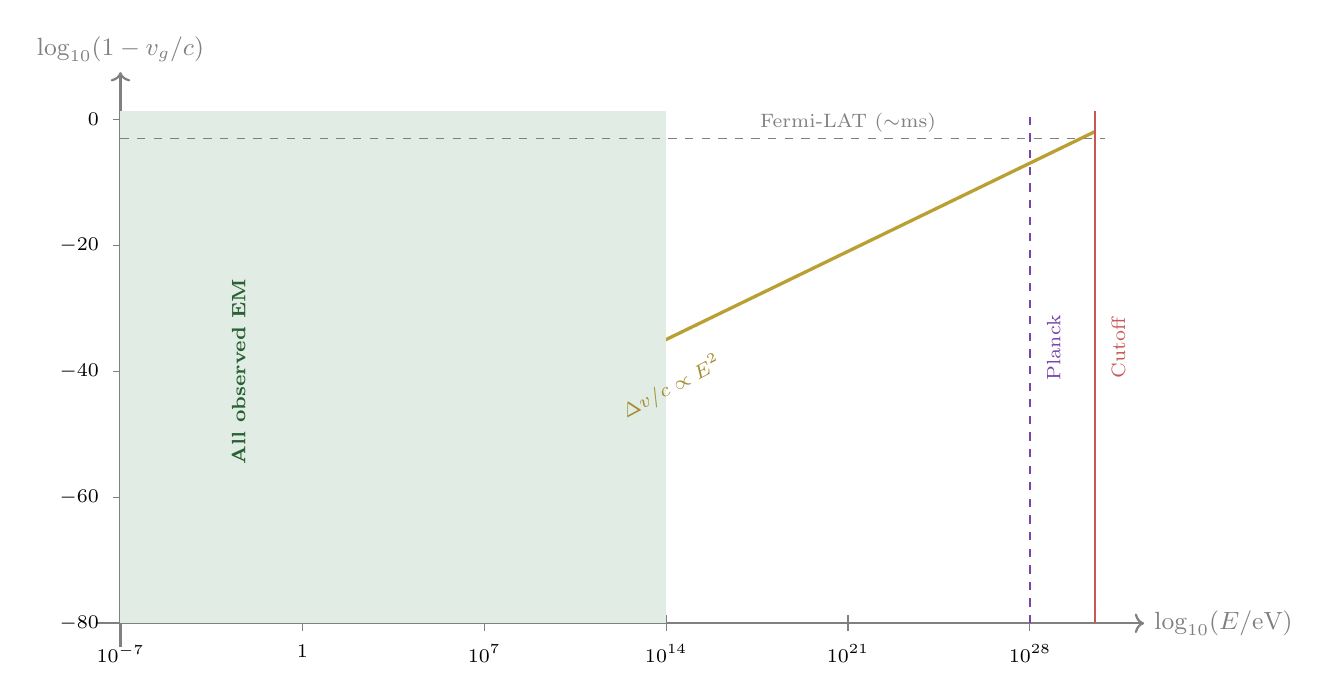
\begin{tikzpicture}[scale=1.0]
  % Manual log-log plot of vacuum dispersion
  % x-axis: log10(E/eV) from -7 to 31
  % y-axis: log10(1 - vg/c) = 2*log10(E) - 62.95
  \def\xscale{0.33}  % cm per decade
  \def\yscale{0.08}  % cm per decade on y

  % Axes
  \draw[->, gray, thick] (-0.3,0) -- (13, 0)
    node[right, font=\small] {$\log_{10}(E/\text{eV})$};
  \draw[->, gray, thick] (0,-0.3) -- (0, 7)
    node[above, font=\small] {$\log_{10}(1 - v_g/c)$};

  % x-axis ticks: E = 10^{-7} to 10^{31} mapped to 0..12.67 cm
  \foreach \e/\lab in {-7/{$10^{-7}$}, 0/{$1$}, 7/{$10^{7}$}, 14/{$10^{14}$},
    21/{$10^{21}$}, 28/{$10^{28}$}} {
    \pgfmathsetmacro{\xp}{(\e+7)*\xscale}
    \draw[gray] (\xp, -0.1) -- (\xp, 0.1);
    \node[font=\scriptsize, below] at (\xp, -0.15) {\lab};
  }

  % y-axis ticks: log10(1-vg/c) from -80 to 0 mapped to 0..6.4
  \foreach \y/\lab in {-80/{$-80$}, -60/{$-60$}, -40/{$-40$}, -20/{$-20$}, 0/{$0$}} {
    \pgfmathsetmacro{\yp}{(\y+80)*\yscale}
    \draw[gray] (-0.1, \yp) -- (0.1, \yp);
    \node[font=\scriptsize, left] at (-0.15, \yp) {\lab};
  }

  % The line: y = 2*x - 62.95 where x = log10(E)
  % At x=-7: y = -76.95 -> yp = 3.05*0.08 = 0.244
  % At x=30.5: y = -1.95 -> yp = 78.05*0.08 = 6.244
  \pgfmathsetmacro{\xa}{(-7+7)*\xscale}
  \pgfmathsetmacro{\ya}{(2*(-7)-62.95+80)*\yscale}
  \pgfmathsetmacro{\xb}{(30.5+7)*\xscale}
  \pgfmathsetmacro{\yb}{(2*30.5-62.95+80)*\yscale}
  \draw[photonyellow!80!black, very thick] (\xa, \ya) -- (\xb, \yb);

  % Green shaded: observed EM (E < 10^14 eV)
  \pgfmathsetmacro{\xobs}{(14+7)*\xscale}
  \fill[bccgreen!15] (0, 0) rectangle (\xobs, 6.5);
  \node[font=\scriptsize\bfseries, bccgreen!70!black, rotate=90] at (1.5, 3.2)
    {All observed EM};

  % Planck energy: E = 1.22e28
  \pgfmathsetmacro{\xpl}{(28+7)*\xscale}
  \draw[bccpurple, thick, dashed] (\xpl, 0) -- (\xpl, 6.5);
  \node[font=\scriptsize, bccpurple, rotate=90] at (\xpl+0.3, 3.5) {Planck};

  % Cutoff: E ~ 3.3e30
  \pgfmathsetmacro{\xcut}{(30.5+7)*\xscale}
  \draw[bccred, thick] (\xcut, 0) -- (\xcut, 6.5);
  \node[font=\scriptsize, bccred, rotate=90] at (\xcut+0.3, 3.5) {Cutoff};

  % Fermi-LAT sensitivity: ~10^{-3} -> log = -3 -> yp = 77*0.08 = 6.16
  \pgfmathsetmacro{\yfermi}{(-3+80)*\yscale}
  \draw[gray, thin, dashed] (0, \yfermi) -- (12.5, \yfermi);
  \node[font=\scriptsize, gray, right] at (8, \yfermi+0.2) {Fermi-LAT ($\sim$ms)};

  % Label
  \node[font=\scriptsize, photonyellow!70!black, rotate=28] at (7, 3.0)
    {$\Delta v/c \propto E^2$};

\end{tikzpicture}
\caption{Vacuum dispersion $1 - v_g/c$ versus photon energy (log-log). The relation is
quadratic: $\Delta v/c \propto E^2$. All observed electromagnetic radiation (green
shaded region) produces deviations far below any conceivable measurement sensitivity.
The lattice becomes visible only near the Planck energy (purple dashed line) and
reaches complete standing-wave cutoff (red solid line) at $E_{\mathrm{cutoff}} = 2\hbar c/a$.}
\label{fig:vacuum-dispersion}
\end{figure}

\subsection{Observational Constraints on the Lattice Spacing}

The Fermi-LAT constrains vacuum dispersion using arrival-time differences of
gamma-ray photons from distant sources. For the quadratic dispersion that a lattice
produces, the constraint is $E_{\mathrm{QG}} \gtrsim 1.3 \times 10^{20}$~eV,
translating to $a \lesssim 3 \times 10^{-30}$~m $\approx 2 \times 10^5\,\ell_P$.
A sub-Planckian lattice ($a \ll \ell_P$) is safely consistent.

\begin{figure}[H]
\centering
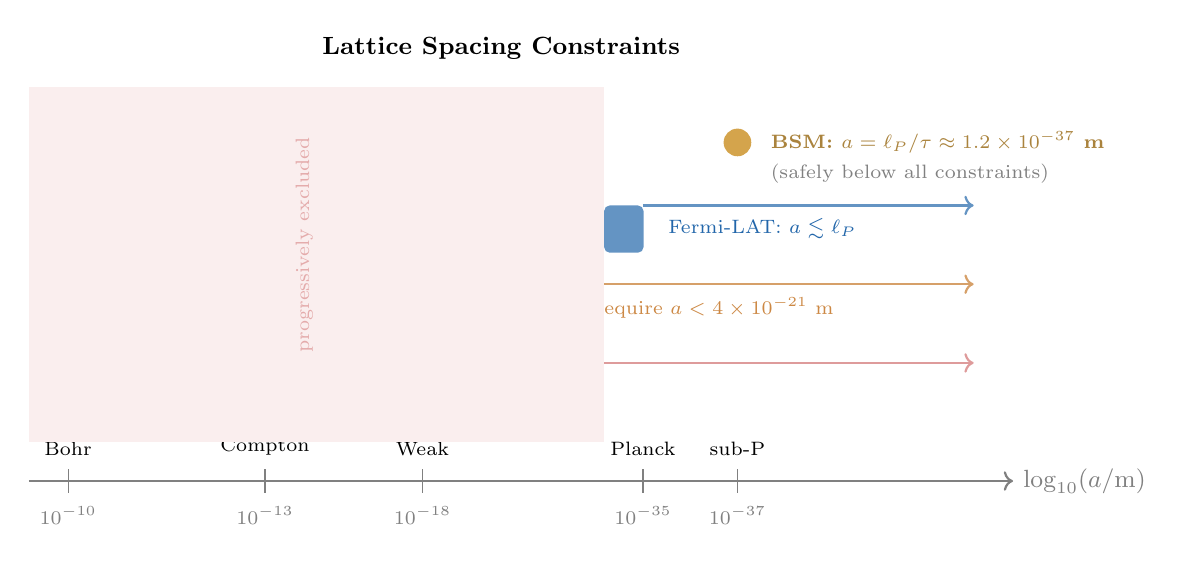
\begin{tikzpicture}[
  bar/.style={rounded corners=2pt, minimum height=0.6cm, anchor=west, font=\footnotesize\bfseries, text=white}
]
  \node[font=\bfseries\small] at (6, 5.5) {Lattice Spacing Constraints};
  \draw[->, gray, thick] (0, 0) -- (12.5, 0) node[right, font=\small] {$\log_{10}(a/\mathrm{m})$};

  % Scale markers
  \foreach \x/\lab/\val in {
    0.5/{Bohr}/{$10^{-10}$},
    3.0/{Compton}/{$10^{-13}$},
    5.0/{Weak}/{$10^{-18}$},
    7.8/{Planck}/{$10^{-35}$},
    9.0/{sub-P}/{$10^{-37}$}
  } {
    \draw[gray] (\x, -0.15) -- (\x, 0.15);
    \node[font=\scriptsize, gray, below] at (\x, -0.2) {\val};
    \node[font=\scriptsize, above] at (\x, 0.2) {\lab};
  }

  % Constraint bars
  % Hard X-rays
  \node[bar, fill=bccred!60, minimum width=0.5cm] at (0.5, 1.2) {};
  \draw[bccred!60, thick, ->] (1.0, 1.5) -- (12, 1.5);
  \node[font=\scriptsize, bccred!80!black, right] at (1.2, 1.2) {Hard X-rays require $a < 4\times10^{-11}$~m};

  % 100 TeV gamma
  \node[bar, fill=vpcol!80, minimum width=0.5cm] at (5.0, 2.2) {};
  \draw[vpcol!80, thick, ->] (5.5, 2.5) -- (12, 2.5);
  \node[font=\scriptsize, vpcol, right] at (5.7, 2.2) {100~TeV $\gamma$ require $a < 4\times10^{-21}$~m};

  % Fermi-LAT
  \node[bar, fill=bccblue!70, minimum width=0.5cm] at (7.3, 3.2) {};
  \draw[bccblue!70, thick, ->] (7.8, 3.5) -- (12, 3.5);
  \node[font=\scriptsize, bccblue, right] at (8.0, 3.2) {Fermi-LAT: $a \lesssim \ell_P$};

  % BSM natural choice
  \fill[bccgold] (9.0, 4.3) circle (5pt);
  \node[font=\scriptsize\bfseries, bccgold!80!black, right] at (9.3, 4.3)
    {BSM: $a = \ell_P/\tau \approx 1.2\times10^{-37}$~m};
  \node[font=\scriptsize, gray, right] at (9.3, 3.9)
    {(safely below all constraints)};

  % Excluded region
  \fill[bccred!10] (0, 0.5) rectangle (7.3, 5.0);
  \node[font=\scriptsize, bccred!50, rotate=90] at (3.5, 3.0) {progressively excluded};

\end{tikzpicture}
\caption{Observational constraints on the lattice spacing $a$. Each constraint
eliminates lattice spacings above its threshold. The BSM natural scale
$a = \ell_P/\tau$ (gold dot) lies far below all observational bounds.}
\label{fig:constraints}
\end{figure}


\subsection{Optical Phenomena from the Lattice}

The lattice accounts for all familiar photon properties:

\begin{photonbox}[Photon Properties from the BCC Lattice]
\begin{description}[nosep, leftmargin=1em, font=\bfseries\small]
  \item[Masslessness] The photon is a gauge mode: the $\mathrm{U}(1)$ phase along a
    bond is a flat direction of the lattice action, protected by gauge invariance.
    $\omega(0) = 0$.
  \item[Polarization] A bond oriented along $\hat{x}$ supports transverse fluctuations
    in $\hat{y}$ and $\hat{z}$: $d - 1 = 2$ polarization states. The longitudinal
    mode is pure gauge.
  \item[Speed of light] $c = \lim_{k\to 0}\omega/k$ is the lattice propagation velocity,
    determined by bond stiffness over inertia per site. Not an external input.
  \item[Bose statistics] The binary defect has $\mathbb{Z}_2$ symmetry (node exchange).
    The longitudinal mode is symmetric $\Rightarrow$ Bose--Einstein statistics.
    Transverse modes are antisymmetric $\Rightarrow$ Fermi--Dirac (leptons).
  \item[Refraction] On the bare lattice, $n_{\mathrm{refr}} = 1$ exactly. Defects
    (matter) produce forward scattering with amplitude $\propto \alpha$, shifting the
    effective phase velocity: $n_{\mathrm{refr}} = 1 + (\text{density}) \times f(\omega)$.
  \item[Diffraction] Native to lattice waves. The photon diffracts identically to
    continuum waves for $\lambda \gg a$.
  \item[Wave--particle duality] \textbf{Wave:} delocalized lattice mode obeying
    $\omega(k)$. \textbf{Particle:} interaction with localized defects at specific sites.
    ``Collapse'' = lattice wave exciting a localized defect.
\end{description}
\end{photonbox}

\begin{figure}[H]
\centering
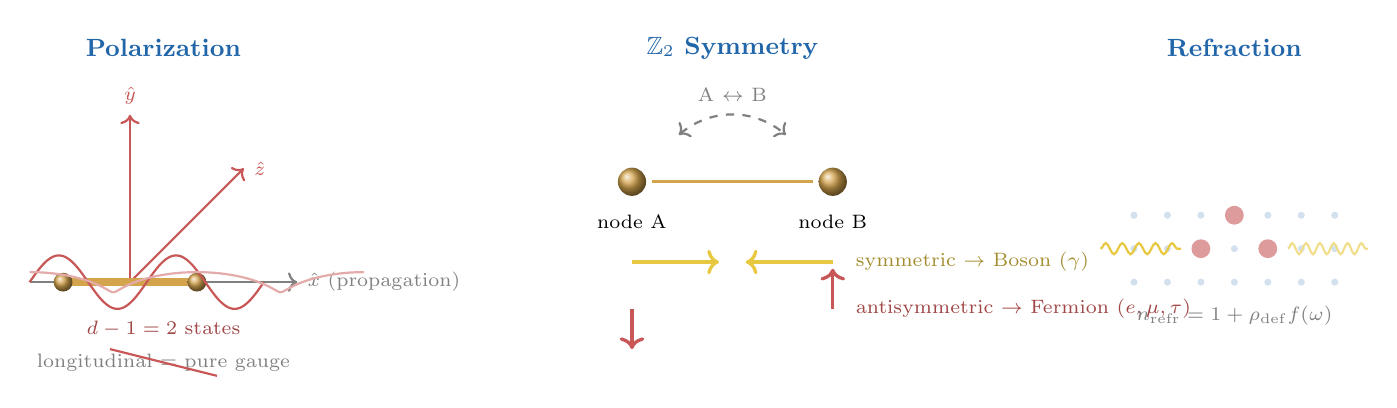
\begin{tikzpicture}[scale=0.85]
  % ── Polarization diagram ──
  \begin{scope}[xshift=-5.5cm]
    \node[font=\bfseries\small, bccblue] at (2, 3.5) {Polarization};
    % Propagation axis
    \draw[->, gray, thick] (0, 0) -- (4, 0) node[right, font=\scriptsize] {$\hat{x}$ (propagation)};
    % Transverse axes
    \draw[->, bccred, thick] (1.5, 0) -- (1.5, 2.5) node[above, font=\scriptsize] {$\hat{y}$};
    \draw[->, bccred, thick] (1.5, 0) -- (3.2, 1.7) node[right, font=\scriptsize] {$\hat{z}$};
    % Bond
    \draw[bccgold, line width=3pt] (0.5, 0) -- (2.5, 0);
    \shade[ball color=bccgold] (0.5,0) circle (4pt);
    \shade[ball color=bccgold] (2.5,0) circle (4pt);
    % Polarization oscillations
    \draw[bccred, thick, smooth, samples=80, domain=0:3.5]
      plot (\x, {0.4*sin(720*\x/3.5)});
    \draw[bccred!50, thick, smooth, samples=80, domain=0:3.5]
      plot ({0.3*sin(720*\x/3.5) + \x + 1.5/3.5*\x},
           {0.3*cos(720*\x/3.5)*0.5});
    \node[font=\scriptsize, bccred!80!black] at (2, -0.7) {$d-1 = 2$ states};
    % Gauge mode crossed out
    \node[font=\scriptsize, gray] at (2, -1.2) {longitudinal = pure gauge};
    \draw[bccred, thick] (1.2, -1.0) -- (2.8, -1.4);
  \end{scope}

  % ── Bose/Fermi from Z2 ──
  \begin{scope}[xshift=3cm]
    \node[font=\bfseries\small, bccblue] at (2, 3.5) {$\mathbb{Z}_2$ Symmetry};
    % Bond with node labels
    \shade[ball color=bccgold] (0.5, 1.5) circle (6pt);
    \node[font=\scriptsize] at (0.5, 0.9) {node A};
    \shade[ball color=bccgold] (3.5, 1.5) circle (6pt);
    \node[font=\scriptsize] at (3.5, 0.9) {node B};
    \draw[bccgold, very thick] (0.8, 1.5) -- (3.2, 1.5);
    % Swap arrow
    \draw[<->, gray, thick, dashed] (1.2, 2.2) to[bend left=40] (2.8, 2.2);
    \node[font=\scriptsize, gray] at (2, 2.8) {A $\leftrightarrow$ B};
    % Symmetric mode
    \draw[photonyellow, very thick, ->] (0.5, 0.3) -- (1.8, 0.3);
    \draw[photonyellow, very thick, ->] (3.5, 0.3) -- (2.2, 0.3);
    \node[font=\scriptsize, photonyellow!70!black, right] at (3.7, 0.3)
      {symmetric $\to$ Boson ($\gamma$)};
    % Antisymmetric mode
    \draw[bccred, very thick, ->] (0.5, -0.4) -- (0.5, -1.0);
    \draw[bccred, very thick, ->] (3.5, -0.4) -- (3.5, 0.2);
    \node[font=\scriptsize, bccred!80!black, right] at (3.7, -0.4)
      {antisymmetric $\to$ Fermion ($e,\mu,\tau$)};
  \end{scope}

  % ── Refraction ──
  \begin{scope}[xshift=11cm]
    \node[font=\bfseries\small, bccblue] at (1.5, 3.5) {Refraction};
    % Vacuum lattice
    \foreach \x in {0,0.5,...,3.0} {
      \fill[bccblue!20] (\x, 0) circle (1.5pt);
      \fill[bccblue!20] (\x, 0.5) circle (1.5pt);
      \fill[bccblue!20] (\x, 1.0) circle (1.5pt);
    }
    % Defects in material
    \fill[bccred!60] (1.0, 0.5) circle (4pt);
    \fill[bccred!60] (2.0, 0.5) circle (4pt);
    \fill[bccred!60] (1.5, 1.0) circle (4pt);
    % Incoming wave
    \draw[photonyellow, thick, decorate, decoration={snake, amplitude=2pt, segment length=6pt}]
      (-0.5, 0.5) -- (0.7, 0.5);
    % Forward scattered
    \draw[photonyellow!60, thick, decorate, decoration={snake, amplitude=2pt, segment length=5pt}]
      (2.3, 0.5) -- (3.5, 0.5);
    \node[font=\scriptsize, gray] at (1.5, -0.5) {$n_{\mathrm{refr}} = 1 + \rho_{\mathrm{def}} f(\omega)$};
  \end{scope}
\end{tikzpicture}
\caption{Optical phenomena on the lattice. \textbf{Left:} Polarization arises from
$d-1 = 2$ transverse oscillation directions; the longitudinal mode is eliminated by
gauge invariance. \textbf{Center:} The $\mathbb{Z}_2$ node-exchange symmetry gives
Bose statistics to the symmetric (photon) mode and Fermi statistics to the
antisymmetric (lepton) modes. \textbf{Right:} Refraction arises from forward scattering
off lattice defects (matter) with amplitude $\propto \alpha$.}
\label{fig:optical}
\end{figure}

\subsection{The Photon--Higgs Connection}

The Higgs boson is the breathing mode of the lattice: uniform oscillation of spacing
$a(t) = \aBCC[1 + h(t)]$, where $h(t)$ is the Higgs field. The photon propagates
\emph{on} this oscillating lattice, making the two modes fundamentally coupled.

If the lattice spacing oscillates, the photon dispersion becomes time-dependent:
$\omega(k,t) \approx ck[1 - h(t)]$. This is parametric phase modulation---the same
mechanism as Brillouin scattering in condensed matter. The modulation depth per site
is $\alpha/\rho$; integrated over the BZ gives $\pi\alpha/\rho = 0.002547$, which is
\emph{exactly} the Higgs VP correction factor.

\begin{figure}[H]
\centering
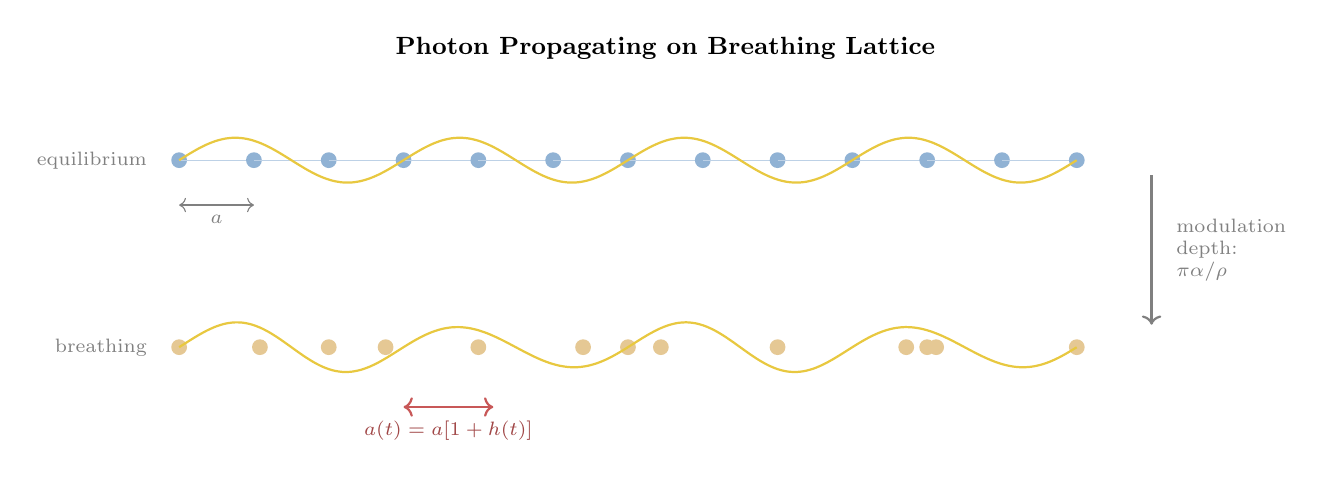
\begin{tikzpicture}[scale=0.95]
  % ── Breathing mode ──
  \node[font=\bfseries\small] at (6.5, 5) {Photon Propagating on Breathing Lattice};

  % Static lattice (top)
  \begin{scope}[yshift=3cm]
    \node[font=\scriptsize, gray, left] at (-0.3, 0.5) {equilibrium};
    \foreach \x in {0,1,...,12} {
      \fill[bccblue!50] (\x, 0.5) circle (3pt);
      \ifnum\x<12
        \draw[bccblue!30] (\x, 0.5) -- (\x+1, 0.5);
      \fi
    }
    % Photon wave
    \draw[photonyellow, thick, smooth, samples=100, domain=0:12]
      plot (\x, {0.5 + 0.3*sin(360*\x/3)});
    \draw[<->, gray, thin] (0, -0.1) -- (1, -0.1) node[midway, below, font=\scriptsize] {$a$};
  \end{scope}

  % Breathing lattice (bottom)
  \begin{scope}[yshift=0.5cm]
    \node[font=\scriptsize, gray, left] at (-0.3, 0.5) {breathing};
    \foreach \x [evaluate=\x as \xpos using \x*(1+0.08*sin(360*\x/4))] in {0,1,...,12} {
      \fill[bccgold!60] (\xpos, 0.5) circle (3pt);
    }
    % Modulated photon wave
    \draw[photonyellow, thick, smooth, samples=100, domain=0:12]
      plot (\x, {0.5 + 0.3*sin(360*\x/3) * (1 + 0.15*sin(360*\x/6))});
    % Breathing indicator
    \draw[<->, bccred, thick] (3, -0.3) -- (4.2, -0.3);
    \node[font=\scriptsize, bccred!80!black, below] at (3.6, -0.35)
      {$a(t) = a[1+h(t)]$};
  \end{scope}

  % Connection to Higgs VP
  \draw[->, thick, gray] (13, 3.3) -- (13, 1.3);
  \node[font=\scriptsize, align=left, gray, right] at (13.2, 2.3)
    {modulation\\depth:\\$\pi\alpha/\rho$};

\end{tikzpicture}
\caption{The photon--Higgs coupling. \textbf{Top:} Photon propagating on a static
lattice (equilibrium spacing $a$). \textbf{Bottom:} The same photon on a breathing
lattice ($a(t) = a[1+h(t)]$). The amplitude modulation is the physical origin of the
Higgs VP correction $\pi\alpha/\rho$. This coupling is intrinsically quantum---it
turns on at one loop through the BZ integral $c_1 = \pi^2/2$.}
\label{fig:photon-higgs}
\end{figure}

\begin{insightbox}[Photon's Channel in the Higgs Mass]
The Standard Model has $d+1 = 4$ gauge bosons ($W^+, W^-, Z, \gamma$). Three
become massive; the photon stays massless because $\mathrm{U}(1)_{\mathrm{EM}}$ is
unbroken. In BSM, the Goldstone subtraction removes $d = 3$ modes (not $d+1$).
The photon's masslessness \emph{raises} the Higgs mass by exactly one dressed
proton mass:
\[
  m_H^{\gamma\,\text{massless}} - m_H^{\gamma\,\text{massive}}
  = \left(1 + \frac{\pi\alpha}{\rho}\right)m_p \approx 940.7~\text{MeV}
\]
The photon contributes one scalar channel to the Higgs sector precisely because
$\mathrm{U}(1)_{\mathrm{EM}}$ is unbroken.
\end{insightbox}


% ══════════════════════════════════════════════════════════════
\section{The Four-Channel Correction Taxonomy}
\label{sec:taxonomy}

Every BSM formula shares a universal four-channel correction structure.

\begin{figure}[H]
\centering
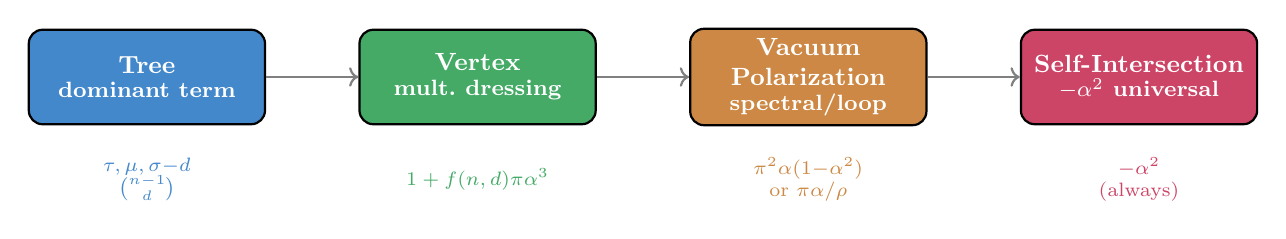
\begin{tikzpicture}[
  channel/.style={rounded corners=5pt, minimum width=3cm, minimum height=1.2cm,
    draw, thick, font=\small\bfseries, text=white, align=center},
  arr/.style={->, thick, gray}
]
  \node[channel, fill=treecol] (tree) at (0, 0) {Tree\\[-2pt]{\footnotesize dominant term}};
  \node[channel, fill=vertexcol] (vert) at (4.2, 0) {Vertex\\[-2pt]{\footnotesize mult.\ dressing}};
  \node[channel, fill=vpcol] (vp) at (8.4, 0) {Vacuum\\Polarization\\[-2pt]{\footnotesize spectral/loop}};
  \node[channel, fill=selfcol] (self) at (12.6, 0) {Self-Intersection\\[-2pt]{\footnotesize $-\alpha^2$ universal}};
  \draw[arr] (tree) -- (vert);
  \draw[arr] (vert) -- (vp);
  \draw[arr] (vp) -- (self);
  \node[font=\scriptsize, treecol, align=center] at (0, -1.3)
    {$\tau, \mu, \sigma{-}d$\\$\binom{n{-}1}{d}$};
  \node[font=\scriptsize, vertexcol, align=center] at (4.2, -1.3)
    {$1 + f(n,d)\pi\alpha^3$};
  \node[font=\scriptsize, vpcol, align=center] at (8.4, -1.3)
    {$\pi^2\alpha(1{-}\alpha^2)$\\or $\pi\alpha/\rho$};
  \node[font=\scriptsize, selfcol, align=center] at (12.6, -1.3)
    {$-\alpha^2$\\(always)};
\end{tikzpicture}
\caption{The universal four-channel correction taxonomy.}
\label{fig:taxonomy}
\end{figure}

\begin{table}[H]
\centering\small
\renewcommand{\arraystretch}{1.4}
\begin{tabular}{l
  >{\columncolor{treecol!10}}c
  >{\columncolor{vertexcol!10}}c
  >{\columncolor{vpcol!10}}c
  >{\columncolor{selfcol!10}}c}
\toprule
\textbf{Observable} & \textbf{Tree} & \textbf{Vertex} & \textbf{VP} & \textbf{Self-int.} \\
\midrule
$\ainv$
  & $\tau = 137$
  & $c_1/\tau, \ldots, c_4/\tau^4$
  & $1/(n{+}2)B^2$
  & (Dyson) \\
$m_p/m_e$
  & $\mu = 1836$
  & $\times(1{+}2(2n{+}1)\pi\alpha^3)$
  & $(1{+}\frac{1}{2n})\pi^2\alpha(1{-}\alpha^2)$
  & $-\alpha^2$ \\
$m_\mu/m_e$
  & $\frac{d}{2}\tau = 205.5$
  & $+\frac{d}{2}\pi\sigma\alpha^3$
  & $\frac{d}{2}\pi\alpha(1{-}\alpha^2)$
  & $-\alpha^2$ \\
$m_\tau/m_e$
  & Koide: $Q = \frac{d-1}{d}$
  & \multicolumn{2}{c}{$\delta Q = \frac{(d{-}1)\pi^2\alpha^2}{(n{-}1)\sigma}$}
  & --- \\
$m_H/m_p$
  & $\sigma - d = 133$
  & ---
  & $\times(1{+}\pi\alpha/\rho)$
  & --- \\
$\Delta m / m_e$
  & $\binom{7}{3}\pi^2\alpha$
  & $\times(1{+}\frac{(n{-}d)\alpha}{\rho})$
  & $\times(1{+}\frac{(n{-}1)\alpha^2}{n{+}2})$
  & $-\alpha^2$ \\
\bottomrule
\end{tabular}
\caption{The correction taxonomy applied to all six BSM observables.}
\label{tab:taxonomy}
\end{table}


% ══════════════════════════════════════════════════════════════
\section{Mass Predictions}
\label{sec:masses}

\subsection{The Proton--Electron Mass Ratio}

The proton is a ternary (3-node) defect with structural parameter $n$:
\begin{equation}
\boxed{
  \frac{m_p}{m_e} = \mu\bigl(1 + 2(2n{+}1)\pi\alpha^3\bigr)
  + \Bigl(1 + \frac{1}{2n}\Bigr)\pi^2\alpha(1{-}\alpha^2) - \alpha^2
}
\label{eq:proton}
\end{equation}
Prediction: $1836.152\,673\,5$ \quad (CODATA: $1836.152\,673\,426(32)$, agreement $< 0.03\ppb$).

\subsection{The Muon--Electron Mass Ratio}

The muon is a binary (2-node) defect excitation with structural parameter $d$:
\begin{equation}
\boxed{
  \frac{m_\mu}{m_e} = \frac{d}{2}\bigl(\tau + \pi\alpha(1{-}\alpha^2)\bigr)
  + \frac{c_1}{4} + \frac{d}{2}\pi\sigma\alpha^3 - \alpha^2
}
\label{eq:muon}
\end{equation}
Prediction: $206.768\,282\,5$ \quad (CODATA: $206.768\,282\,7(46)$, agreement $1.1\ppb$).


\subsection{The Tau Lepton and the Generation Problem}

The tau mass emerges from the Koide relation, identified as the transverse fraction
of a line defect:
\begin{equation}
\boxed{
  Q \equiv \frac{m_e + m_\mu + m_\tau}{(\sqrt{m_e} + \sqrt{m_\mu} + \sqrt{m_\tau})^2}
  = \frac{d-1}{d} + \frac{(d{-}1)\pi^2\alpha^2}{(n{-}1)\sigma}
}
\label{eq:koide}
\end{equation}

\begin{figure}[H]
\centering
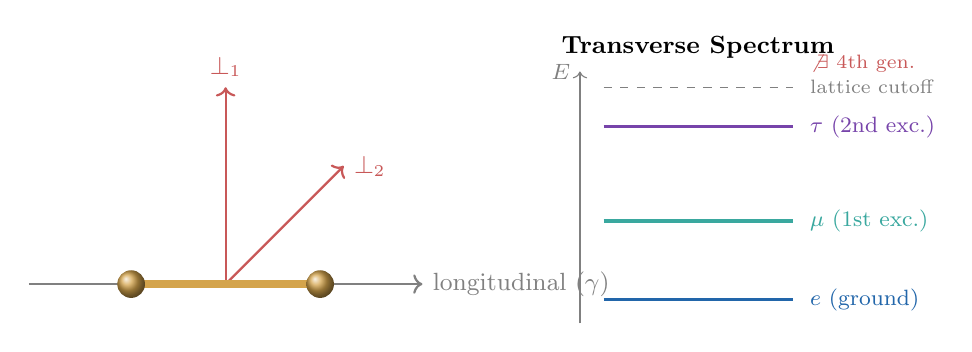
\begin{tikzpicture}[scale=1.0]
  % The line defect in 3D
  \draw[->, gray, thick] (-0.5,0) -- (4.5,0) node[right, font=\small] {longitudinal ($\gamma$)};
  \draw[->, bccred, thick] (2,0) -- (2,2.5) node[above, font=\small] {$\perp_1$};
  \draw[->, bccred, thick] (2,0) -- (3.5,1.5) node[right, font=\small] {$\perp_2$};
  \draw[bccgold, line width=3pt] (0.8,0) -- (3.2,0);
  \shade[ball color=bccgold] (0.8,0) circle (5pt);
  \shade[ball color=bccgold] (3.2,0) circle (5pt);

  % Transverse oscillator levels
  \begin{scope}[xshift=6.5cm, yshift=-0.5cm]
    \node[font=\bfseries\small] at (1.5,3.5) {Transverse Spectrum};
    \draw[->, gray] (0,0) -- (0,3.2) node[left, font=\footnotesize] {$E$};
    \draw[bccblue, very thick] (0.3, 0.3) -- (2.7, 0.3);
    \draw[bccteal, very thick] (0.3, 1.3) -- (2.7, 1.3);
    \draw[bccpurple, very thick] (0.3, 2.5) -- (2.7, 2.5);
    \draw[gray, dashed] (0.3, 3.0) -- (2.7, 3.0);
    \node[font=\scriptsize, gray, right] at (2.8, 3.0) {lattice cutoff};
    \node[font=\footnotesize, bccblue, right] at (2.8, 0.3) {$e$ (ground)};
    \node[font=\footnotesize, bccteal, right] at (2.8, 1.3) {$\mu$ (1st exc.)};
    \node[font=\footnotesize, bccpurple, right] at (2.8, 2.5) {$\tau$ (2nd exc.)};
    \node[font=\scriptsize, bccred, right] at (2.8, 3.3) {$\not\exists$ 4th gen.};
  \end{scope}
\end{tikzpicture}
\caption{The binary defect and its transverse spectrum. Three bound states
(electron, muon, tau) with no fourth generation.}
\label{fig:binary-transverse}
\end{figure}

\noindent
Prediction: $m_\tau/m_e = 3477.4799$ \quad (CODATA: $3477.48 \pm 0.57$, agreement $0.027\ppm$).


\subsection{The Higgs Boson Mass}

The Higgs is the breathing mode. Of $\sigma = 136$ pairwise scalar modes,
$d = 3$ become Goldstone bosons, leaving $\sigma - d = 133$:
\begin{equation}
\boxed{
  \frac{m_H}{m_p} = (\sigma - d)\left(1 + \frac{\pi\alpha}{\rho}\right)
  = 133 \times 1.002547 = 133.339
}
\label{eq:higgs}
\end{equation}

\begin{figure}[H]
\centering
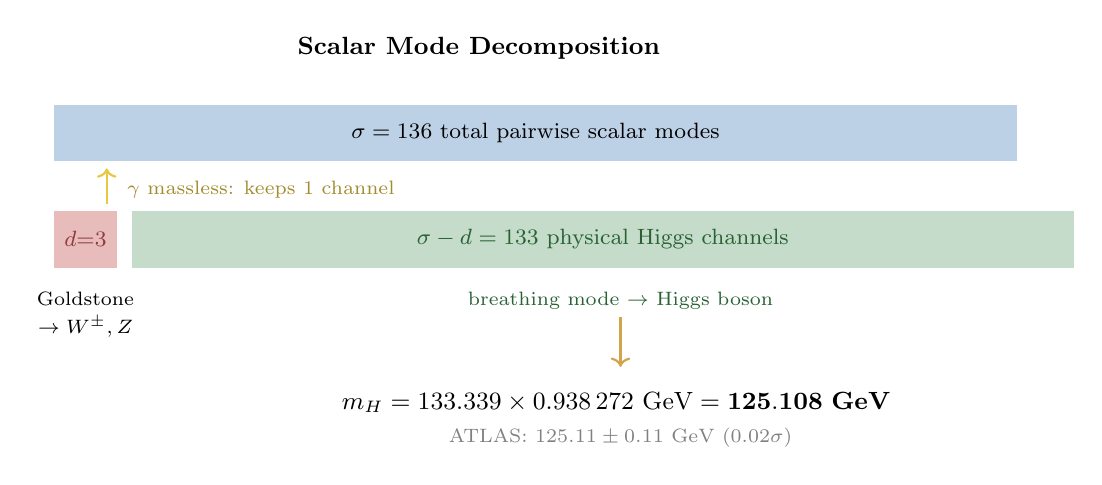
\begin{tikzpicture}[scale=0.9]
  \node[font=\bfseries\small] at (6, 4.8) {Scalar Mode Decomposition};
  \fill[bccblue!30] (0,3.2) rectangle (13.6, 4.0);
  \node[font=\footnotesize] at (6.8, 3.6) {$\sigma = 136$ total pairwise scalar modes};
  \fill[bccred!40] (0, 1.7) rectangle (0.3*3, 2.5);
  \node[font=\footnotesize, bccred!70!black] at (0.45, 2.1) {$d{=}3$};
  \node[font=\scriptsize, below] at (0.45, 1.5) {Goldstone};
  \node[font=\scriptsize, below] at (0.45, 1.15) {$\to W^\pm, Z$};
  \fill[bccgreen!30] (1.1, 1.7) rectangle (1.1+0.1*133, 2.5);
  \node[font=\footnotesize, bccgreen!70!black] at (1.1+6.65, 2.1) {$\sigma - d = 133$ physical Higgs channels};
  \node[font=\scriptsize, below, bccgreen!70!black] at (8, 1.5) {breathing mode $\to$ Higgs boson};
  % Photon channel callout
  \draw[photonyellow, thick, ->] (0.75, 2.6) -- (0.75, 3.1);
  \node[font=\scriptsize, photonyellow!70!black, right] at (0.9, 2.8)
    {$\gamma$ massless: keeps 1 channel};
  \draw[->, thick, bccgold] (8, 1.0) -- (8, 0.3);
  \node[font=\small, align=center] at (8, -0.2) {
    $m_H = 133.339 \times 0.938\,272~\text{GeV} = \mathbf{125.108}$~\textbf{GeV}
  };
  \node[font=\scriptsize, gray] at (8, -0.7) {ATLAS: $125.11 \pm 0.11$~GeV (0.02$\sigma$)};
\end{tikzpicture}
\caption{Higgs mass from scalar mode decomposition. The photon's masslessness means
$d=3$ (not $d+1=4$) modes are eaten, raising the Higgs mass by one dressed proton mass.}
\label{fig:higgs}
\end{figure}


\subsection{The Neutron--Proton Mass Difference}

\begin{equation}
\boxed{
  \frac{\Delta m}{m_e} = \binom{n{-}1}{d}\pi^2\alpha
  \left(1 + \frac{(n{-}d)\alpha}{\rho} - \alpha^2\right)
  \times \left(1 + \frac{(n{-}1)\alpha^2}{n{+}2}\right)
}
\label{eq:neutron}
\end{equation}
Prediction: $2.531\,029\,91\,m_e$ \quad (Experiment: $2.531\,030\,00(3)\,m_e$,
agreement $0.036\ppm$).

% ══════════════════════════════════════════════════════════════
\section{The VP Catalog and Self-Consistency Loop}
\label{sec:vp}

\begin{figure}[H]
\centering
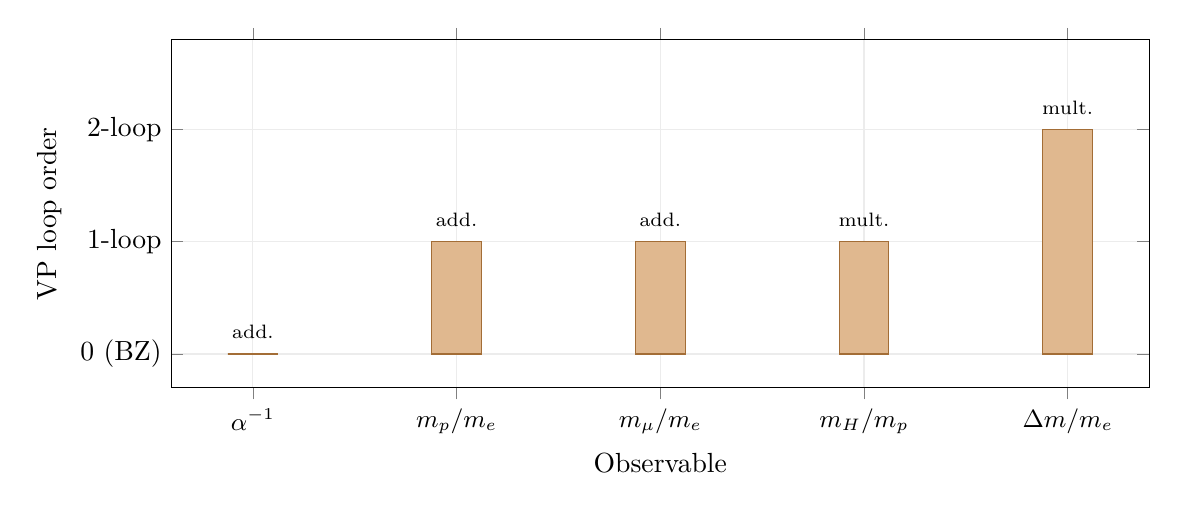
\begin{tikzpicture}
\begin{axis}[
  width=14cm, height=6cm,
  ybar, bar width=18pt,
  xlabel={Observable},
  ylabel={VP loop order},
  ymin=-0.3, ymax=2.8,
  xtick={1,2,3,4,5},
  xticklabels={$\ainv$, $m_p/m_e$, $m_\mu/m_e$, $m_H/m_p$, $\Delta m/m_e$},
  x tick label style={font=\small},
  ytick={0,1,2},
  yticklabels={0 (BZ), 1-loop, 2-loop},
  grid=major, grid style={gray!15},
  nodes near coords,
  every node near coord/.append style={font=\scriptsize, above, yshift=2pt},
  point meta=explicit symbolic
]
  \addplot[fill=vpcol!60, draw=vpcol!80!black] coordinates {
    (1, 0) [{\scriptsize add.}]
    (2, 1) [{\scriptsize add.}]
    (3, 1) [{\scriptsize add.}]
    (4, 1) [{\scriptsize mult.}]
    (5, 2) [{\scriptsize mult.}]
  };
\end{axis}
\end{tikzpicture}
\caption{VP loop-order hierarchy. Each VP lives one loop above its tree level.}
\label{fig:vp-catalog}
\end{figure}


The photon participates in a closed self-consistency loop:

\begin{figure}[H]
\centering
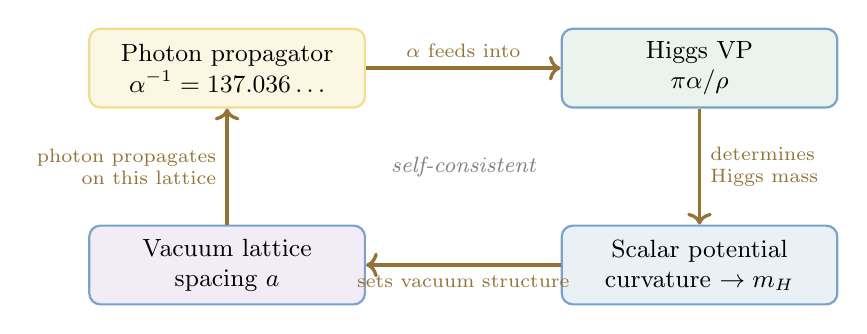
\begin{tikzpicture}[
  box/.style={rounded corners=4pt, draw=bccblue!60, thick, fill=bccblue!8,
    minimum width=3.5cm, minimum height=1.0cm, font=\small, align=center},
  arr/.style={->, very thick, bccgold!70!black}
]
  \node[box, fill=photonyellow!15, draw=photonyellow!60] (photon) at (0, 0)
    {Photon propagator\\$\ainv = 137.036\ldots$};
  \node[box, fill=bccgreen!10] (higgs) at (6, 0)
    {Higgs VP\\$\pi\alpha/\rho$};
  \node[box, fill=bccblue!10] (scalar) at (6, -2.5)
    {Scalar potential\\curvature $\to m_H$};
  \node[box, fill=bccpurple!10] (lattice) at (0, -2.5)
    {Vacuum lattice\\spacing $a$};

  \draw[arr] (photon) -- node[above, font=\scriptsize] {$\alpha$ feeds into} (higgs);
  \draw[arr] (higgs) -- node[right, font=\scriptsize, align=left] {determines\\Higgs mass} (scalar);
  \draw[arr] (scalar) -- node[below, font=\scriptsize] {sets vacuum structure} (lattice);
  \draw[arr] (lattice) -- node[left, font=\scriptsize, align=right] {photon propagates\\on this lattice} (photon);

  \node[font=\footnotesize\itshape, gray] at (3, -1.25) {self-consistent};
\end{tikzpicture}
\caption{The photon self-consistency loop. The same $\alpha$ that emerges from the
Dyson equation enters the Higgs VP and produces a scalar potential whose curvature
yields the lattice on which $\alpha$ is defined.}
\label{fig:self-consistency}
\end{figure}


% ══════════════════════════════════════════════════════════════
\section{Complete Scorecard}
\label{sec:scorecard}

\begin{table}[H]
\centering
\renewcommand{\arraystretch}{1.3}
\begin{tabular}{lcccl}
\toprule
\textbf{Constant} & \textbf{BSM Prediction} & \textbf{Experiment} & \textbf{Agreement} & \textbf{Origin} \\
\midrule
$\ainv$ & $137.035\,999\,177$ & $137.035\,999\,177(21)$ & $<0.001\ppb$ & photon propagator \\
$m_p/m_e$ & $1836.152\,673\,5$ & $1836.152\,673\,426(32)$ & $<0.03\ppb$ & ternary defect ($n$) \\
$m_\mu/m_e$ & $206.768\,282\,5$ & $206.768\,282\,7(46)$ & $1.1\ppb$ & binary defect ($d$) \\
$m_\tau/m_e$ & $3477.4799$ & $3477.48 \pm 0.57$ & $0.027\ppm$ & Koide (transverse) \\
$m_H/m_p$ & $133.339$ & $133.34(12)$ & $0.02\sigma$ & breathing mode \\
$\Delta m/m_e$ & $2.531\,029\,91$ & $2.531\,030\,00(3)$ & $0.036\ppm$ & ternary orient. \\
\bottomrule
\end{tabular}
\caption{Six fundamental constants from two inputs ($n = 8$, $\pi$) plus $d = 3$. Zero free parameters.}
\label{tab:scorecard}
\end{table}


% ══════════════════════════════════════════════════════════════
\section{Structural Architecture}
\label{sec:architecture}

\begin{figure}[H]
\centering
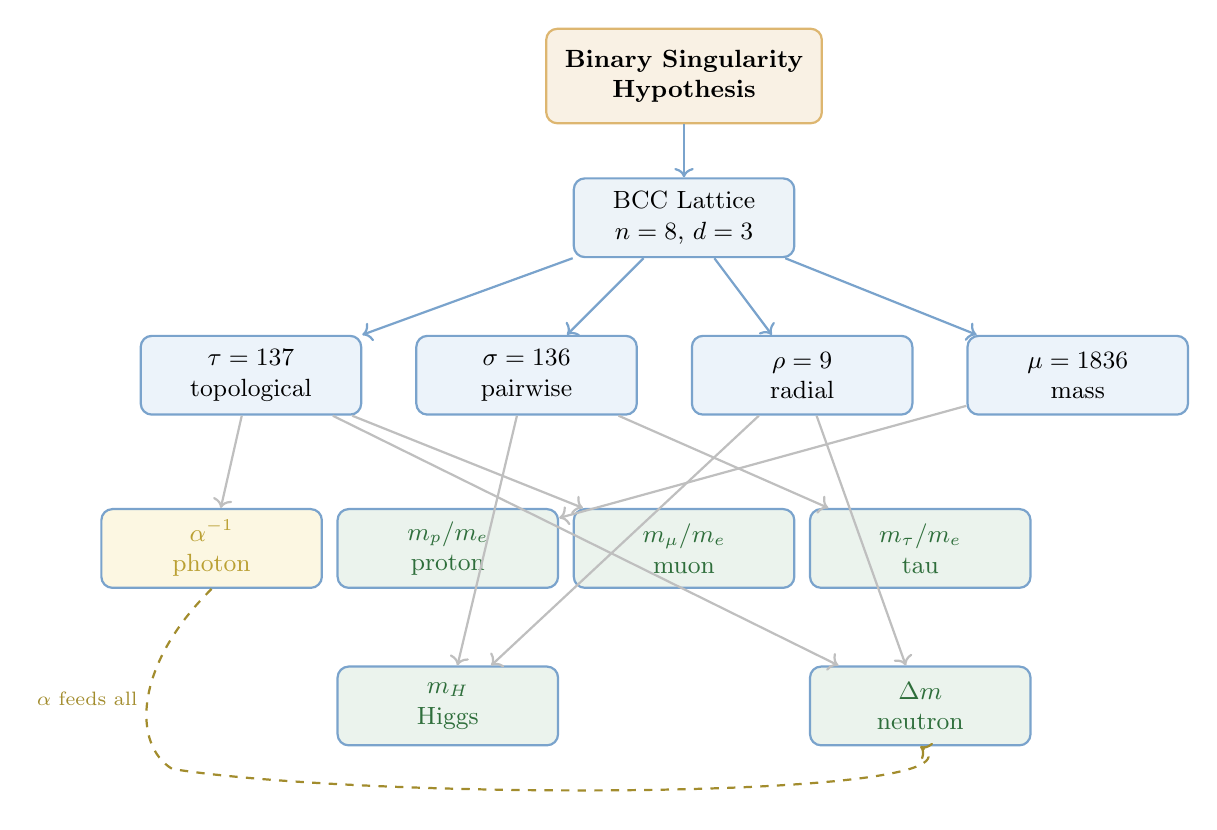
\begin{tikzpicture}[
  box/.style={rounded corners=4pt, draw=bccblue!60, thick, fill=bccblue!8,
    minimum width=2.8cm, minimum height=1.0cm, font=\small, align=center},
  bigbox/.style={rounded corners=4pt, draw=bccgold!80, thick, fill=bccgold!8,
    minimum width=3.5cm, minimum height=1.2cm, font=\small\bfseries, align=center},
  arr/.style={->, thick, bccblue!60}
]
  \node[bigbox, fill=bccgold!15] (hyp) at (6, 8) {Binary Singularity\\Hypothesis};
  \node[box] (bcc) at (6, 6.2) {BCC Lattice\\$n = 8$, $d = 3$};
  \draw[arr] (hyp) -- (bcc);
  \node[box, fill=treecol!10] (tau) at (0.5, 4.2) {$\tau = 137$\\topological};
  \node[box, fill=treecol!10] (sig) at (4, 4.2) {$\sigma = 136$\\pairwise};
  \node[box, fill=treecol!10] (rho) at (7.5, 4.2) {$\rho = 9$\\radial};
  \node[box, fill=treecol!10] (mu) at (11, 4.2) {$\mu = 1836$\\mass};
  \draw[arr] (bcc) -- (tau); \draw[arr] (bcc) -- (sig);
  \draw[arr] (bcc) -- (rho); \draw[arr] (bcc) -- (mu);

  % Observables
  \node[box, fill=photonyellow!15, text=photonyellow!80!black] (alp) at (0, 2.0) {$\ainv$\\photon};
  \node[box, fill=bccgreen!10, text=bccgreen!80!black] (pro) at (3, 2.0) {$m_p/m_e$\\proton};
  \node[box, fill=bccgreen!10, text=bccgreen!80!black] (muo) at (6, 2.0) {$m_\mu/m_e$\\muon};
  \node[box, fill=bccgreen!10, text=bccgreen!80!black] (taul) at (9, 2.0) {$m_\tau/m_e$\\tau};
  \node[box, fill=bccgreen!10, text=bccgreen!80!black] (hig) at (3, 0.0) {$m_H$\\Higgs};
  \node[box, fill=bccgreen!10, text=bccgreen!80!black] (neu) at (9, 0.0) {$\Delta m$\\neutron};

  \draw[arr, gray!50] (tau) -- (alp); \draw[arr, gray!50] (mu) -- (pro);
  \draw[arr, gray!50] (tau) -- (muo); \draw[arr, gray!50] (sig) -- (taul);
  \draw[arr, gray!50] (sig) -- (hig); \draw[arr, gray!50] (rho) -- (hig);
  \draw[arr, gray!50] (tau) -- (neu); \draw[arr, gray!50] (rho) -- (neu);

  % Self-consistent alpha feedback
  \draw[->, thick, photonyellow!70!black, dashed] (alp.south) .. controls (-1, 0.5) and (-1, -0.5) ..
    node[left, font=\scriptsize, photonyellow!70!black] {$\alpha$ feeds all} (-0.5, -0.8)
    .. controls (2, -1.2) and (10, -1.2) .. (neu.south);
\end{tikzpicture}
\caption{The BSM architectural flow. The photon's $\alpha$ (yellow, highlighted)
self-consistently feeds into all other predictions.}
\label{fig:architecture}
\end{figure}


% ══════════════════════════════════════════════════════════════
\section{Falsifiability and Predictions}
\label{sec:predictions}

\begin{resultbox}[Higgs Mass Prediction --- Falsifiable at the HL-LHC]
\begin{center}
\renewcommand{\arraystretch}{1.2}
\begin{tabular}{lcc}
\toprule
\textbf{If HL-LHC converges to} & \textbf{BSM deviation} & \textbf{Status} \\
\midrule
$125.11$~GeV (ATLAS) & $0.1\sigma$ & \textcolor{bccgreen}{\textbf{Confirmed}} \\
$125.20$~GeV (world avg.) & $4.4\sigma$ & \textcolor{bccgold}{\textbf{Strongly disfavored}} \\
$125.35$~GeV (CMS) & $11.5\sigma$ & \textcolor{bccred}{\textbf{Ruled out}} \\
\bottomrule
\end{tabular}
\end{center}
\end{resultbox}

\noindent
Structural predictions subject to computational verification:
\begin{enumerate}[nosep]
  \item The transverse Laplacian $D_\perp^2$ on the binary defect has exactly 3 bound
    states (3 lepton generations from geometry).
  \item Lattice perturbation theory at one loop on BCC with $g^2 = 1/2$,
    $N_D = 4$ reproduces $c_1/\tau = \pi^2/(2 \times 137)$.
  \item The scalar effective potential on BCC yields tree-level gap $\sigma - d = 133$.
  \item Vacuum dispersion is quadratic ($\propto E^2$), undetectable for $a \lesssim \ell_P$.
\end{enumerate}


% ══════════════════════════════════════════════════════════════
\section{Photon Summary}
\label{sec:photon-summary}

\begin{table}[H]
\centering\small
\begin{tabular}{lp{9.5cm}}
\toprule
\textbf{Property} & \textbf{BSM lattice account} \\
\midrule
Identity & Longitudinal propagation mode of the binary defect; $\mathrm{U}(1)$ gauge mode on bonds \\
Coupling & $\alpha$ = dressed photon propagator (Dyson equation, $<0.001\ppb$) \\
Masslessness & Gauge invariance: flat direction of lattice action along bond \\
Polarization & $d - 1 = 2$ transverse fluctuations of the bond \\
Speed of light & Lattice propagation velocity $c = \lim_{k\to 0}\omega/k$ \\
Dispersion & $\omega = (2c/a)|\sin(ka/2)|$; linear for $\lambda \gg a$, deviates near $\lambda \sim a$ \\
Statistics & Bose: $\mathbb{Z}_2$-symmetric mode of the two-node defect \\
Refraction & Forward scattering off lattice defects (matter) with amplitude $\sim\alpha$ \\
Higgs coupling & Photon propagates on breathing lattice; coupling $= \pi\alpha/\rho$ \\
Scale constraint & Observation requires $a \lesssim \ell_P$ (sub-Planckian) \\
\bottomrule
\end{tabular}
\caption{Complete photon characterization in the BSM framework.}
\label{tab:photon-summary}
\end{table}


% ══════════════════════════════════════════════════════════════
\section{Open Problems}
\label{sec:open}

\begin{enumerate}[label=(\alph*)]
  \item \textbf{First-principles derivation.} Derive all six formulas from the BCC lattice
    Lagrangian.
  \item \textbf{Photon self-energy.} Compute the one-loop $\Sigma(p)$ on BCC with $g^2=1/2$,
    $N_D = 4$ and verify $c_1/\tau = \pi^2/(2\times 137)$.
  \item \textbf{BCC dispersion.} The exact photon dispersion on BCC (direction-dependent
    velocities, multiple branches) has not been computed from the Dirac operator.
  \item \textbf{Absolute energy scale.} The framework predicts dimensionless ratios but not
    the Higgs vev $v = 246$~GeV or any absolute mass in GeV.
  \item \textbf{$H\to\gamma\gamma$ coupling.} The Higgs--photon--photon vertex exists through
    the breathing-mode modulation with coupling $\sim\alpha/(\sigma-d)$, but an explicit
    branching ratio has not been derived.
  \item \textbf{Electroweak sector.} The Goldstone subtraction connects to $W^\pm, Z$ but
    does not yet predict the Weinberg angle or gauge boson mass ratios.
  \item \textbf{Graviton.} If the photon is the $\mathrm{U}(1)$ mode on bonds, is there a
    spin-2 mode on plaquettes or higher simplices identifiable with the graviton?
  \item \textbf{Quark sector and gravity.} Can the defect classification extend to quarks and
    the sub-Planckian origin connect to quantum gravity?
\end{enumerate}

\vfill

\begin{center}
\small\itshape
``Two sub-Planckian singularities in orbit. A lattice with eight neighbors.\\
Six constants from two inputs and a transcendental.\\
The photon is the most precisely predicted object in the framework---\\
and the object whose question started it all.''
\end{center}

\end{document}
